
%%%%%%%%%%%%%%%%%%%%%%%%%%%%%%%%%%%%%%%%%%%%%%%%%%%%%%%%%%%%%%%%%%%%%%%%%%%%%%
%                                                                            %
%  ************************** AVISO IMPORTANTE **************************    %
%                                                                            %
% Éste es un documento de ayuda para los autores que deseen enviar           %
% trabajos para su consideración en el Boletín de la Asociación Argentina    %
% de Astronomía.                                                             %
%                                                                            %
% Los comentarios en este archivo contienen instrucciones sobre el formato   %
% obligatorio del mismo que complementan los instructivos web y PDF.         %
% Por favor léalos.                                                          %
%                                                                            %
% No deben borrarse los comentarios en este archivo. En caso contrario,      %
% el sistema de recepción de manuscritos no permitirá el envío de su         %
% contribución. No se permite el uso de \newcommand ni definiciones          %
% particulares de cada autor.                                                %
%                                                                            %
%%%%%%%%%%%%%%%%%%%%%%%%%%%%%%%%%%%%%%%%%%%%%%%%%%%%%%%%%%%%%%%%%%%%%%%%%%%%%%

%%%%%%%%%%%%%%%%%%%%%%%%%%%%%%%%%%%%%%%%%%%%%%%%%%%%%%%%%%%%%%%%%%%%%%%%%%%%%%
%                                                                            %
%  ************************** IMPORTANT NOTICE **************************    %
%                                                                            %
%  This is a help file for authors who are preparing manuscripts to be       %
%  considered for publication in the Boletín de la Asociación Argentina      %
%  de Astronomía.                                                            %
%                                                                            %
%  The comments in this file give instructions about the manuscripts'        %
%  mandatory format that complement the instructions distributed as a PDF    %
%  and findable in the BAAA web. Please read them.                           %
%                                                                            %
%  The comments in this file must not be deleted. Otherwise, your            %
%  contribution will be rejected by the manuscript reception system.         %
%  The use of \newcommand and author definitions are forbidden.              %
%                                                                            %
%%%%%%%%%%%%%%%%%%%%%%%%%%%%%%%%%%%%%%%%%%%%%%%%%%%%%%%%%%%%%%%%%%%%%%%%%%%%%%

\documentclass[baaa]{baaa}

\usepackage[pdftex]{hyperref}
\usepackage{subfigure}
\usepackage{natbib}
\usepackage{helvet,soul}
\usepackage[font=small]{caption}

%%%%%%%%%%%%%%%%%%%%%%%%%%%%%%%%%%%%%%%%%%%%%%%%%%%%%%%%%%%%%%%%%%%%%%%%%%%%%%
%                                                                            %
%  Seleccione el idioma de su contribución: Recuerde que todos los           %
%  componentes del documento (titulo, texto, figuras, tablas, etc.)          %
%  deben estar en el mismo idioma.                                           %
%                                                                            %
%  Select the language of your contribution: Please remember that all       %
%  document parts (title, text, figures, tables, etc.) must be in the        %
%  same language.                                                            %
%                                                                            %
%  0: Castellano / Spanish                                                   %
%  1: Inglés / English                                                       %
%                                                                            %
%%%%%%%%%%%%%%%%%%%%%%%%%%%%%%%%%%%%%%%%%%%%%%%%%%%%%%%%%%%%%%%%%%%%%%%%%%%%%%

\contriblanguage{0}

%%%%%%%%%%%%%%%%%%%%%%%%%%%%%%%%%%%%%%%%%%%%%%%%%%%%%%%%%%%%%%%%%%%%%%%%%%%%%%
%                                                                            %
%  Seleccione el tipo de contribución solicitada:                            %
%                                                                            %
%  Select the requested contribution type:                                   %
%                                                                            %
%  1: Presentación mural / Poster                                            %
%  2: Presentación oral / Oral contribution                                  %
%  3: Informe invitado / Invited report                                      %
%  4: Mesa redonda / Round table                                             %
%  5: Presentación Premio Varsavsky / Varsavsky Prize contribution           %
%  6: Presentación Premio Sahade / Sahade Prize contribution                 %
%  7: Presentación Premio Sérsic / Sérsic Prize contribution                 %
%                                                                            %
%%%%%%%%%%%%%%%%%%%%%%%%%%%%%%%%%%%%%%%%%%%%%%%%%%%%%%%%%%%%%%%%%%%%%%%%%%%%%%

\contribtype{2}

%%%%%%%%%%%%%%%%%%%%%%%%%%%%%%%%%%%%%%%%%%%%%%%%%%%%%%%%%%%%%%%%%%%%%%%%%%%%%%
%                                                                            %
%  Seleccione el área temática de su contribución:                           %
%                                                                            %
%  Select the thematic area of your contribution:                            %
%                                                                            %
%  1 [AEC]:   Astrofísica Extragaláctica y Cosmología /                      %
%             Extragalactic Astrophysics and Cosmology                       %
%  2 [EG]:    Estructura Galáctica / Galactic Structure                      %
%  3 [AE]:    Astrofísica Estelar / Stellar Astrophysics                     %
%  4 [SE]:    Sistemas Estelares / Stellar Systems                           %
%  5 [ICSA]:  Instrumentación y Caracterización de Sitios Astronómicos /     %
%             Instrumentation and Astronomical Site Characterization         %
%  6 [MI]:    Medio Interestelar / Interstellar Medium                       %
%  7 [OCPAE]: Objetos Compactos y Procesos de Altas Energías /               %
%             Compact Objetcs and High-Energy Processes                      %
%  8 [SH]:    Sol y Heliosfera / Sun and Heliosphere                         %
%  9 [SSE]:   Sistemas Solar y Extrasolares / Solar and Extrasolar Systems   %
% 10 [HEDA]:  Historia, Enseñanza y Divulgación de la Astronomía /           %
%             History, Teaching and Spreading of Astronomy                   %
% 11 [O]:     Otros / Other Topics                                           %
%                                                                            %
%%%%%%%%%%%%%%%%%%%%%%%%%%%%%%%%%%%%%%%%%%%%%%%%%%%%%%%%%%%%%%%%%%%%%%%%%%%%%%

\thematicarea{8}

\title{Estudio de Validación Tomográfica del modelo MHD AWSoM}
%\subtitle{Instrucciones de estilo}

%%%%%%%%%%%%%%%%%%%%%%%%%%%%%%%%%%%%%%%%%%%%%%%%%%%%%%%%%%%%%%%%%%%%%%%%%%%%%%
%                                                                            %
%  Agregue un título corto para el encabezado de las páginas pares.          %
%                                                                            %
%  Add a short title to appear in the header of even pages.                  %
%                                                                            %
%%%%%%%%%%%%%%%%%%%%%%%%%%%%%%%%%%%%%%%%%%%%%%%%%%%%%%%%%%%%%%%%%%%%%%%%%%%%%%

\titlerunning{Macro BAAA61B con instrucciones de estilo}

%%%%%%%%%%%%%%%%%%%%%%%%%%%%%%%%%%%%%%%%%%%%%%%%%%%%%%%%%%%%%%%%%%%%%%%%%%%%%%
%                                                                            %
%  Lista de autores. Los nombres de los autores deben estar separados por    %
%  comas, y deben tener el formato A.E. Autor (iniciales apellido(s); sin    %
%  coma entre apellido e iniciales ni espacios entre las iniciales).         %
%                                                                            %
%  Author list. Authors' names must be separated by commas, and stick to     %
%  the format A.E. Author (initials Family name -neither commas between      %
%  name and the initials nor blanks between the initials).                   %
%                                                                            %
%%%%%%%%%%%%%%%%%%%%%%%%%%%%%%%%%%%%%%%%%%%%%%%%%%%%%%%%%%%%%%%%%%%%%%%%%%%%%%

\author{D.G. Lloveras\inst{1}, A.M. Vásquez\inst{1}, F.A. Nuevo\inst{1}, C. Mac Cormack\inst{1}, N. Sachdeva\inst{2},\\ W. Manchester IV\inst{2}, B. Van der Holst\inst{2}, \& R.A. Frazin\inst{2}}
\authorrunning{Lloveras et al.}


%%%%%%%%%%%%%%%%%%%%%%%%%%%%%%%%%%%%%%%%%%%%%%%%%%%%%%%%%%%%%%%%%%%%%%%%%%%%%%
%                                                                            %
% Por favor provea una dirección de e-mail de contacto para los lectores.    %
%                                                                            %
% Please provide a contact e-mail address for the readers.                   %
%                                                                            %
%%%%%%%%%%%%%%%%%%%%%%%%%%%%%%%%%%%%%%%%%%%%%%%%%%%%%%%%%%%%%%%%%%%%%%%%%%%%%%

\contact{dlloveras@iafe.uba.ar}

\institute{
Insituto de Astronomía y Física del Espacio, CONICET--UBA, Argentina \and
Climate and Space Sciences and Engineering, Universidad de Michigan, EEUU.
}

%%%%%%%%%%%%%%%%%%%%%%%%%%%%%%%%%%%%%%%%%%%%%%%%%%%%%%%%%%%%%%%%%%%%%%%%%%%%%%
%                                                                            %
%  El resumen y el abstract son ambos obligatorios, independientemente del   %
%  lenguaje elegido.                                                         %
%                                                                            %
%  The Resumen and the abstract are both mandatory, regardless of the chosen %
%  language.                                                                 %
%                                                                            %
%%%%%%%%%%%%%%%%%%%%%%%%%%%%%%%%%%%%%%%%%%%%%%%%%%%%%%%%%%%%%%%%%%%%%%%%%%%%%%

\resumen{
Los modelos magnetohidrodinámicos (MHD) tridimensionales (3D),  necesarios para modelar y predecir el clima espacial, deben ser validados observacionalmente. A escala global, esto puede ser hecho mediante tomografía de medida de emisión diferencial (DEMT), que provee resultados 3D de densidad y temperatura electrónica en la baja corona ($1.0-1.25 \, \rm{R}_\odot$). Realizamos una validación DEMT de la versión mas reciente del Alfvén Wave Solar Model (AWSoM) del Space Weather Modeling Framework (SWMF). Se lleva a cabo un análisis comparativo a lo largo de las líneas de campo de la densidad y temperatura electrónicas del modelo y la tomografía, así como de cantidades energéticas integrales. Para este estudio se seleccionaron dos rotaciones de mínimo solar, una entre los ciclos solares (SC) 23 y 24, y otra entre los SCs 24 y 25. Discutimos las diferencias observadas entre el modelo y los productos tomográficos, y las limitaciones y posibles mejoras futuras para el modelo AWSoM.)
}

%Discutimos las diferencias observadas ente el modelo y los productos tomográficos, y las limitaciones y posibles mejoras futuras para el modelo AWSoM (no me deja poner mas lineas!)
\abstract{
Aiming model and forecast the space climate, the tri-dimensional (3D) magnetohydrodinamic (MHD) models are in need of observational validations. This can be done using the differential emission measure technique (DEMT) which provides 3D results of electronic density and temperature in the low corona ($1.0-1.25 \, \rm{R}_\odot$). We performed a DEMT validation of the last version of the Alfvén Wave Solar Model (AWSoM) within the Space Weather Modeling Framework (SWMF). We carried out a comparative analysis along de magnetic field lines using thermodynamic quantities of the model and the tomography results. In this study we selected two rotations othe solar minimum between solar cicle (SC) 23 and 24, and the other one between SCs 24 and 25. We discuss the difference observed between the model and the observations, the limitations and the possible upgrades to the AWSOM model.)
}

%%%%%%%%%%%%%%%%%%%%%%%%%%%%%%%%%%%%%%%%%%%%%%%%%%%%%%%%%%%%%%%%%%%%%%%%%%%%%%
%                                                                            %
%  Seleccione las palabras clave que describen su contribución. Las mismas   %
%  son obligatorias, y deben tomarse de la lista de la American Astronomical %
%  Society (AAS), que se encuentra en la página web indicada abajo.          %
%                                                                            %
%  Select the keywords that describe your contribution. They are mandatory,  %
%  and must be taken from the list of the American Astronomical Society      %
%  (AAS), which is available at the webpage quoted below.                    %
%                                                                            %
%  https://aas.org/authors/astronomical-subject-keywords-update-august-2013  %
%                                                                            %
%%%%%%%%%%%%%%%%%%%%%%%%%%%%%%%%%%%%%%%%%%%%%%%%%%%%%%%%%%%%%%%%%%%%%%%%%%%%%%

\keywords{Sun: corona — Sun: fundamental parameters — Sun: UV radiation — Sun: abundances}

\begin{document}

\maketitle

\section{Introducción}
\label{S_intro}
La observación y el modelado de la Corona solar resulta de gran relevancia para el entendimiento de la relación Sol-Tierra, ya que en la Corona es donde el viento solar es calentado, acelerado y tienen lugar eventos impulsivos como eyecciones de masa coronal, flares, etc.
Predecir eventos de clima espacial y sus efectos geomagnéticos requieren modelos 3D precisos de la atmósfera solar basados en la física que se extiende desde la cromósfera, pasando por la corna, hasta la heliosfera. Estos modelos han evolucionado mucho a lo largo de los años, y conforme lo hacen necesitan ser validados mediante nuevas observaciones y mas detalladas comparaciones.

En el presente trabajo nos focalizaremos en el modelo MHD coronal y de viento solar  Alfvén Wave Solar atmosphere Model (AWSoM) que forma parte del space weather Modeling framework (SWMF) \citet{Toth_2012}. El modelo utiliza calentamiento por ondas de Alfvén para proveer un modelo físico descriptivo 3D auto consistente de calentamiento coronal y aceleración de viento solar \citet{sokolov_2013}  \citet{vander_2014}.

A medida que el modelo adopta nuevas mejoras es necesario contrastar los resultados con observaciones. En una reciente publicación \citet{sachdeva_2019} se llevó a cabo una validación de la última versión del modelo para la rotación de Carrington CR2208 y CR2209 con datos \rm{in situ} de ACE, Wind, SDO/AIA, Ulysses, SOHO/LASCO, IPS y OMNI. Los datos de AIA fueron procesados con la técnica tomográfica de \rm{medida de emisión diferencial local} (DEMT) \citep{frazin_2009} la cual permite obtener una distribución 3D de densidad y temperaturas electronicas dentro del rango 1.0 - 1.25${\rm R_\odot}$. Llevaron a cabo comparaciones globales calculando la diferencia relativa pixel a pixel $RD = \frac{X_{AWSoM}}{X_{DEMT}}-1$ a alturas constantes tanto para para $N_e$ como para $T_e$ y se mostró que el modelo es capaz de reproducir las observaciones dentro de un $\sim 20-30\%$. 

Debido a que la corona es gobernada por el campo magnético, resulta de particular interés analizar  la termodinámica de líneas de campo asociadas a distintas estructuras magnéticas (Streamer, Agujero coronal, etc.). Con esta idea en mente presentamos en este trabajo el primer esfuerzo de validación del modelo AWSoM en la baja corona comparando la termodinámica con un modelo semi empírico (DEMT) en distintas estructuras magnéticas. Para esto se seleccionó la rotación CR2082 correspondiente al mínimo de actividad solar del 2009 y una rotación de la fase de  declinacion actual CR2208 (septiembre 2018).


\section{Método}

El modelo AWSOM utiliza magnetogramas synopticos de ADAPT-GONG \citep{arge_2010} como condiciones de contorno en la fotósfera y permite obtener una estructura 3D de parámetros físicos (densidad y temperatura electrónica entre otros) entre 1.0${\rm R_\odot}$ y 1 UA. El modelo presenta una region de transición extendida desde la fotósfera hasta $\sim$ 1.05${\rm R_\odot}$, región que no se tuvo en cuenta en la comparación.

Por otro lado el modelo DEMT utiliza como datos una serie temporal de imágenes EUV cubriendo media rotación solar permitiendo reconstruir la emisividad en forma 3D en la baja corona. Combinando la emisividad de todas las bandas del telescopio se obtiene la \rm{medida de emisión diferencial local} (LDEM). Esta medida es una descripcion cualitativa de la distribución térmica del plasma en cada celda de la grilla 3D de dimension 0.01${\rm R_\odot}$ en dirección radial y 2$^{\circ}$ en latitud y longitud.

En el presente trabajo se utilizaron imagenes obtenidas con STEREO/EUVI-A y SDO/AIA para CR2082 y CR2208 respectivamente. La selección es debido a que ambos períodos presentan baja actividad coronal, mostrando una corona altamente axysimétrica con agujeros coronales en la zona polar y un streamer dominante en las latitudes ecuatoriales. Las imagnes de EUVI estan afectadas de \rm{contaminación de luz dispersa} que fue removida aplicando a cada imagen una \rm{función dispersión del punto} aplicada a cada pixel, para una explicacion mas detallada sobre el método y el impacto en la reconstrucción tomográfica referirse a \citet{shearer_2012} y \citet{lloveras_ba2017}. Para las imágenes de AIA no existe al momento de la escritura de este artículo una función de dispersión adecuada pero se estima que los telescopios de esta generación se ven menos afectados por esta contaminación.

Para llevar a cabo una comparación termodinámica a lo largo de lineas magnéticas se utilizó el campo dado por el modelo MHD. El modelo usa como condición de contorno el magnetograma y como condición inicial el modelo potencial con superficie fuente (PFSS) obtenido resolviendo la ecuacion de Laplace, considerando campo radial en 2.5${\rm R_\odot}$ y luego evolucionandolo en el tiempo \citep{vander_2010}. Los resultados termodinámicos de DEMT y AWSoM son trazados a lo largo de las líneas de campo dentro de la grilla 3D. 



%%%%%%%%%%%%%%%%%%%%%%%%%%%%%%%%%%%%%%%%%%%%%%%%%%%%%%%%%%%%%%%%%%%%%%%%%%%%%%
%                                                                            %
% Para figuras de dos columnas use \begin{figure*} ... \end{figure*}         %
%                                                                            %
%%%%%%%%%%%%%%%%%%%%%%%%%%%%%%%%%%%%%%%%%%%%%%%%%%%%%%%%%%%%%%%%%%%%%%%%%%%%%%


\section{Resultados}
Como ejemplo de los productos tomográficos y del modelo MHD, mostramos en la Figura \ref{fig-carrington} cortes a una altura media de densidad y temperatura electrónica para ambos modelos y ambas rotaciones seleccionadas. La línea negra sólida demarca la frontera entre las líneas magnéticas abiertas (zona polar) de las íneas cerradas (zona ecuatorial). En los mapas de DEMT las celdas negras rempresentan celdas no reconstruidas por la técnica y fueron excluidas del análisis.

Estos mapas muestran rotaciones altamente axysimétricas con estructuras de $N_e$ y $T_e$ modeladas satisfactoriamente tanto en morfología como orden de magnitud.

$N_e$ y $T_e$ es trazada a lo largo de las líneas magnéticas. Los loops cerrados son separados en dos piernas desde la base hasta el ápice. Para cada linea abierta y cada pierna cerrada $N_e(r)$ fue ajustada a una solución hydrostática isotérmica y una escala de altura $\lambda_n$ es determinada. Las variaciones de temperatura con la altura son mas suaves y su promedia a lo largo de las lineas fue determinado para obtener un valor característico. Para este trabajo se tomó en consideración como subselección de estructuras magnéticas las regiones de los agujeros coronales (líneas abiertas) y la del streamer ecuatorial (líneas cerradas), una mas detallada selección de estructuras puede encontrarse en \citet{lloveras_2017}. 



*pearson de temp p-valor
*
Como ejemplo, la Figura \ref{fig-histos} muestra distribución estadística de los resultados DEMT y AWSoM para cada subregion seleccionada. Mientras que $\lambda_n$ es consistente con las observaciones, AWSoM presenta diferencias $<30\%$ en $\left<T_m\right>$ y $N_e$ según la rotación. Similares diferencias se observaron en los agujeros coronales.



\begin{figure*}
  \centering
  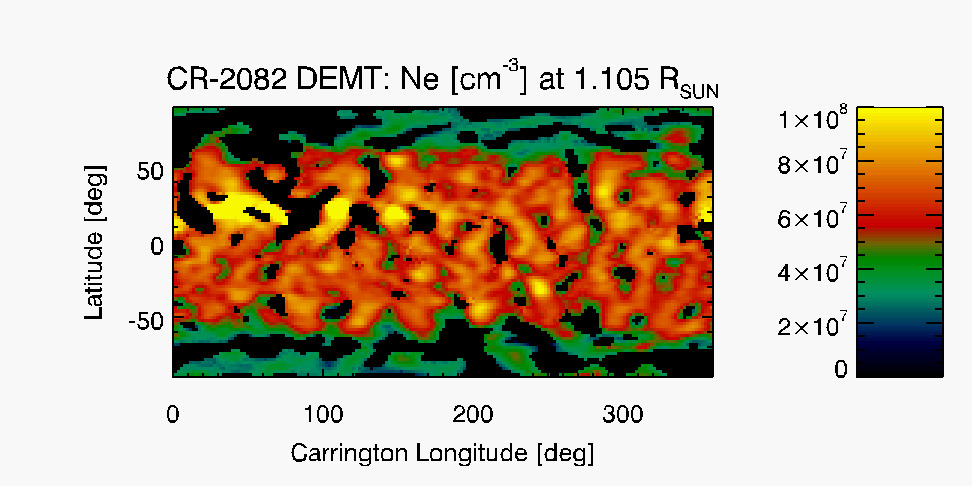
\includegraphics[width=0.4\textwidth]{figuras/map_Ne_CR2082_DEMT-EUVI_behind_H1-L3523_r3d_1105_Rsun.jpg}
  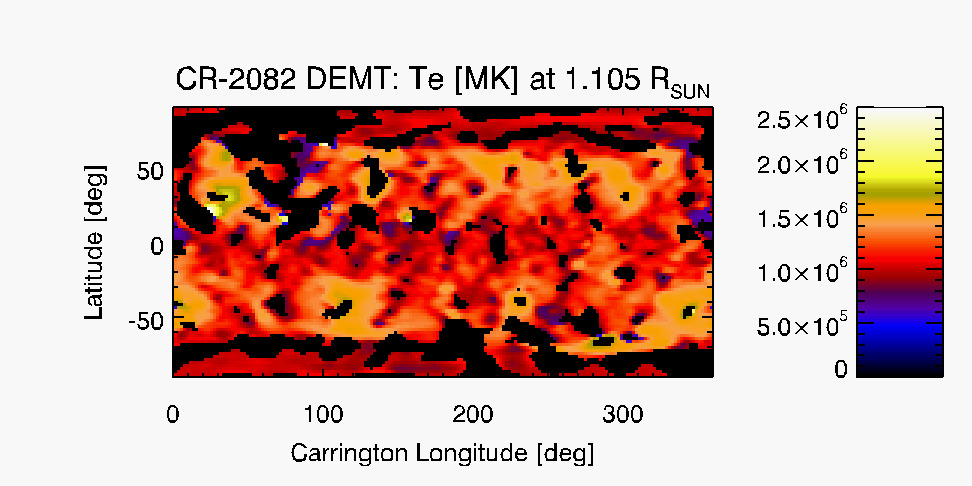
\includegraphics[width=0.4\textwidth]{figuras/map_Tm_CR2082_DEMT-EUVI_behind_H1-L3523_r3d_1105_Rsun.jpg}
  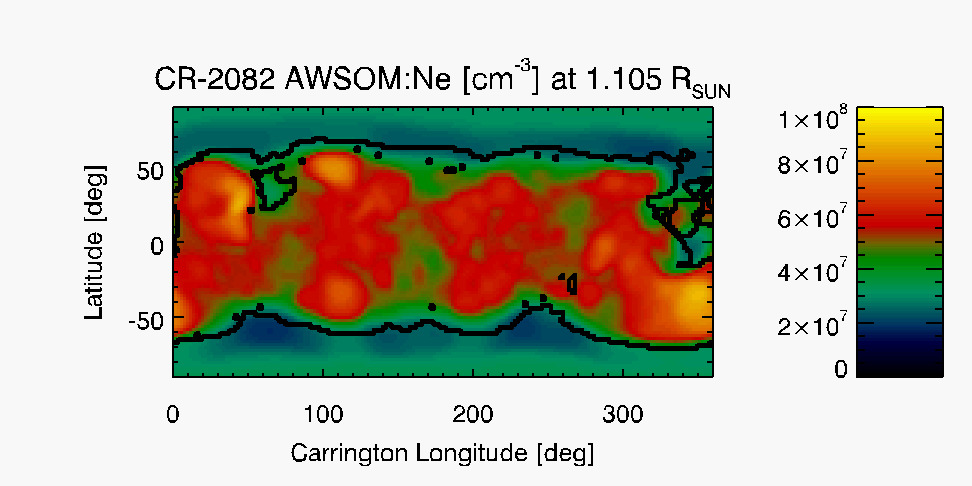
\includegraphics[width=0.4\textwidth]{figuras/map_Ne_awsom_2082_185_short_1105_Rsun.jpg}
  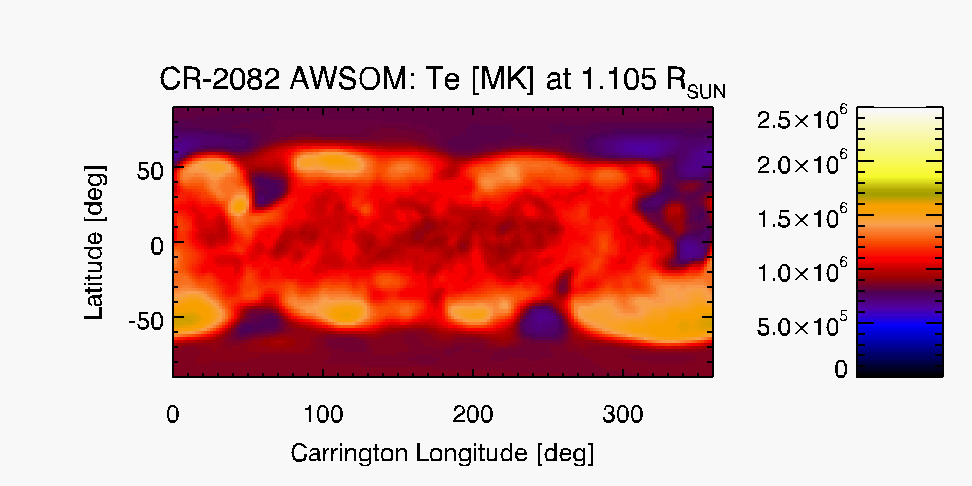
\includegraphics[width=0.4\textwidth]{figuras/map_Te_awsom_2082_185_short_1105_Rsun.jpg}
  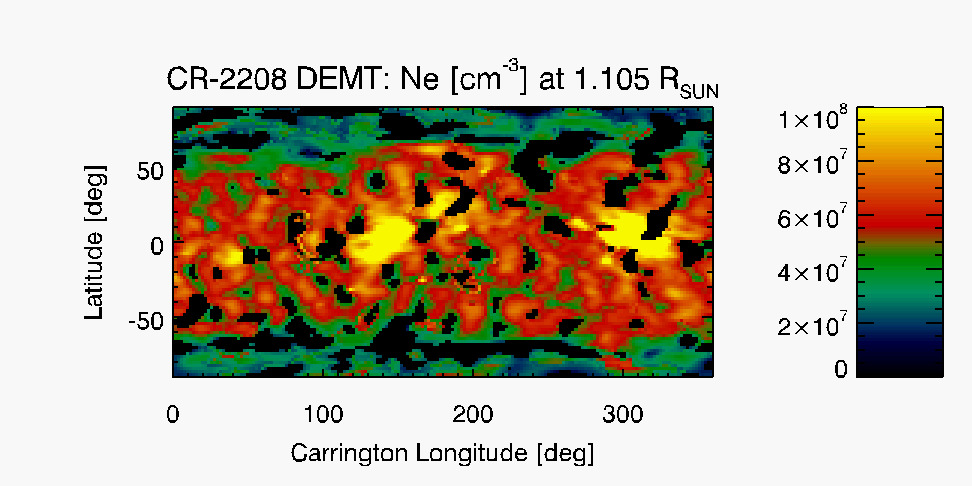
\includegraphics[width=0.4\textwidth]{figuras/map_Ne_CR2208_DEMT-AIA_H1_L522_r3d_1105_Rsun.jpg}
  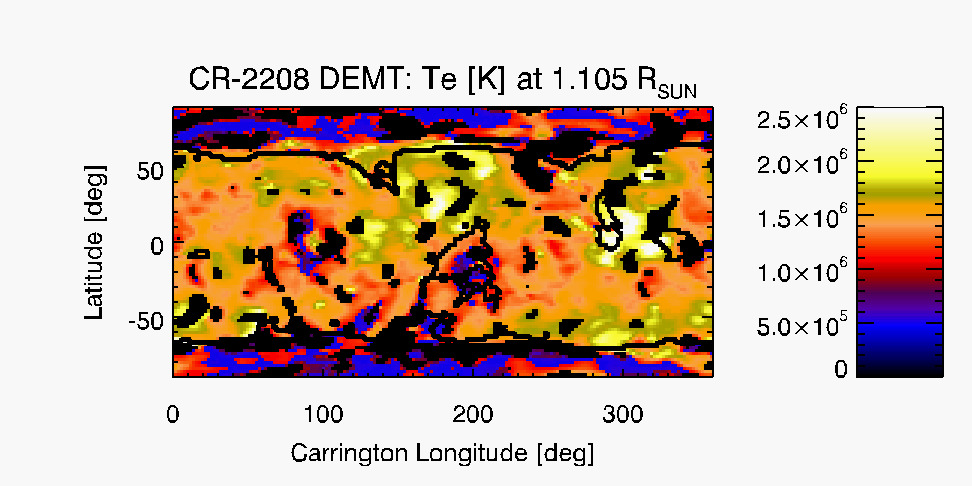
\includegraphics[width=0.4\textwidth]{figuras/map_Tm_CR2208_DEMT-AIA_H1_L522_r3d_1105_Rsun.jpg}  
  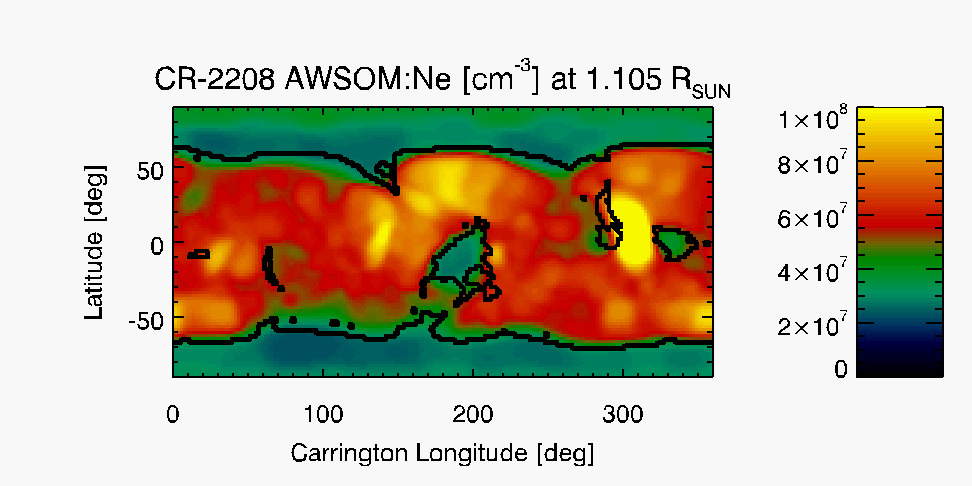
\includegraphics[width=0.4\textwidth]{figuras/map_Ne_awsom_2208_185_short_1105_Rsun.jpg}
  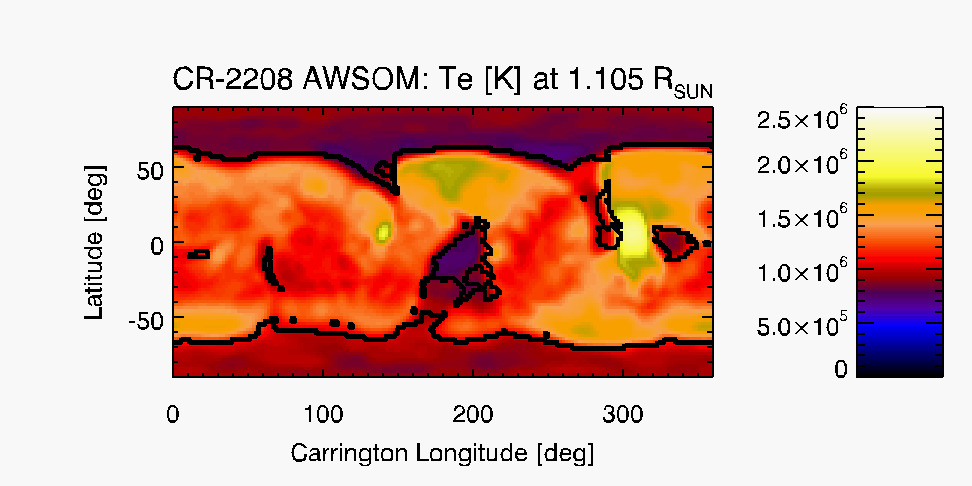
\includegraphics[width=0.4\textwidth]{figuras/map_Te_awsom_2208_185_short_1105_Rsun.jpg}
    \caption{Mapas de Carrington de $T_e$ (derecha) y $N_e$ (izquierda) de CR-2082 y CR-2208 a 1.105 ${\rm R_\odot}$ obtenidas con DEMT y con AWSoM. Las celdas negras corresponden a regiones no reconstruidas, mientras que la curva negra indica el límite de las region magnéticamente abierta en los polos de la magnéticamete cerrada en el Streamer y es obtenida utilizando AWSoM.}
  \label{fig-carrington}
\end{figure*}


%\begin{figure*}
%  \centering
%  \includegraphics[width=0.4\textwidth]{figuras/Midpoint_2082_demt-proceeding_Rpoint-map.eps}
%  \includegraphics[width=0.4\textwidth]{figuras/Midpoint_2208_demt-proceeding_Rpoint-map.eps}
%  \caption{Lolcalización física de los arcos magnéticos a 1.075 ${\rm R_\odot}$. En amarillo la región cerrada y en violeta la región abierta.}
%  \label{fig-rpoint}
%\end{figure*}

\begin{figure*}
  \centering
  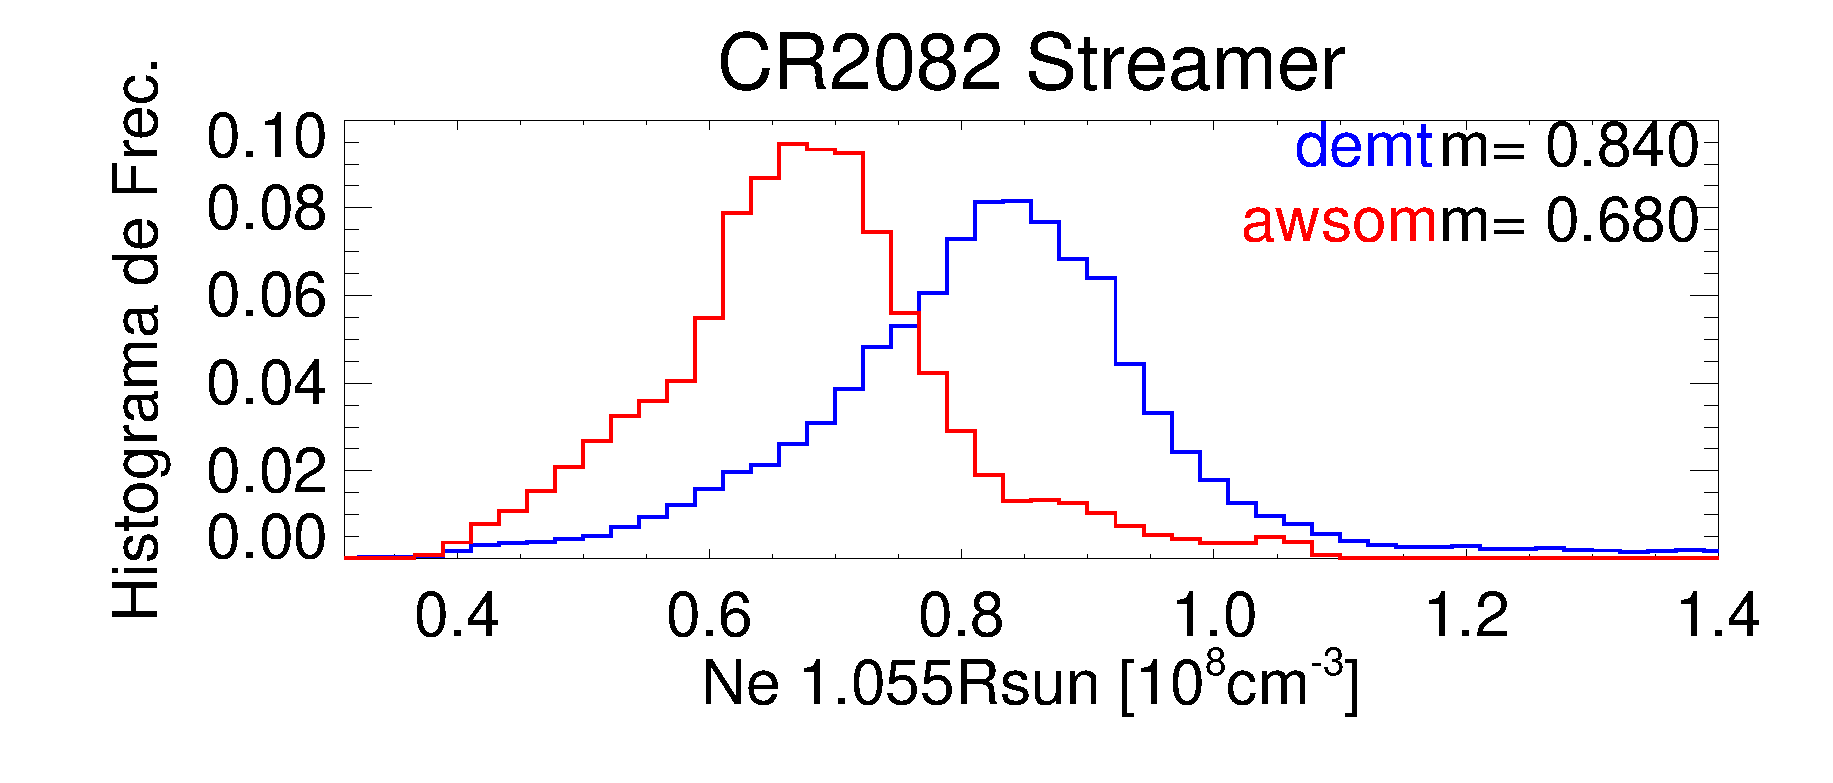
\includegraphics[width=0.32\textwidth]{figuras/proceeding_2082_demt_awsom_streamer_ne_1055.eps}
  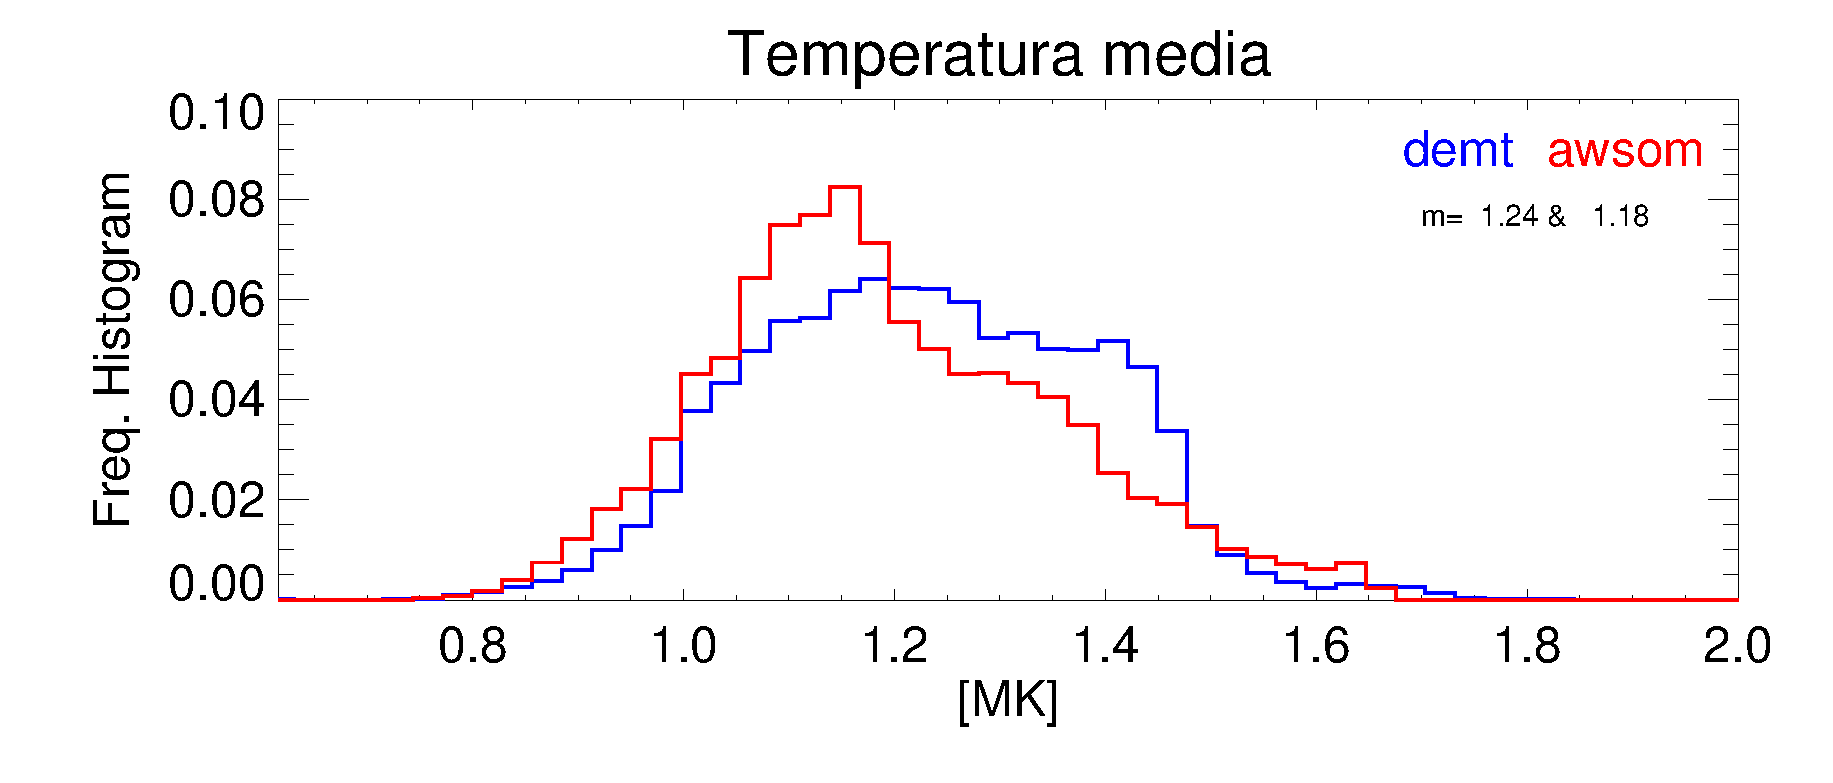
\includegraphics[width=0.32\textwidth]{figuras/proceeding_2082_demt_awsom_streamer_Tm.eps}
  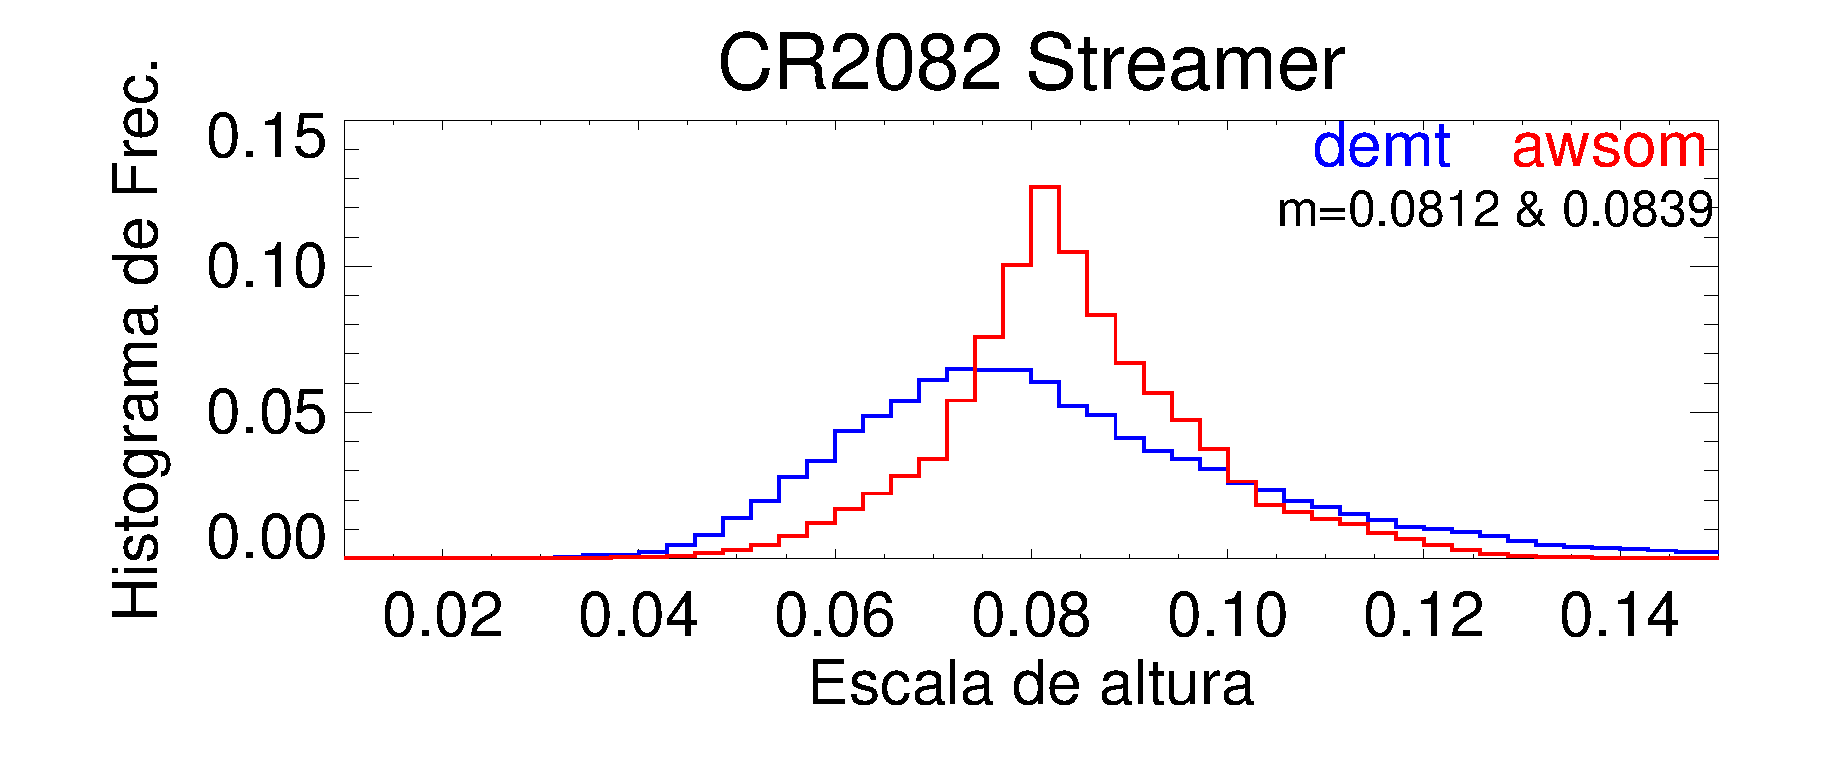
\includegraphics[width=0.32\textwidth]{figuras/proceeding_2082_demt_awsom_streamer_lambda_n.eps}\\
  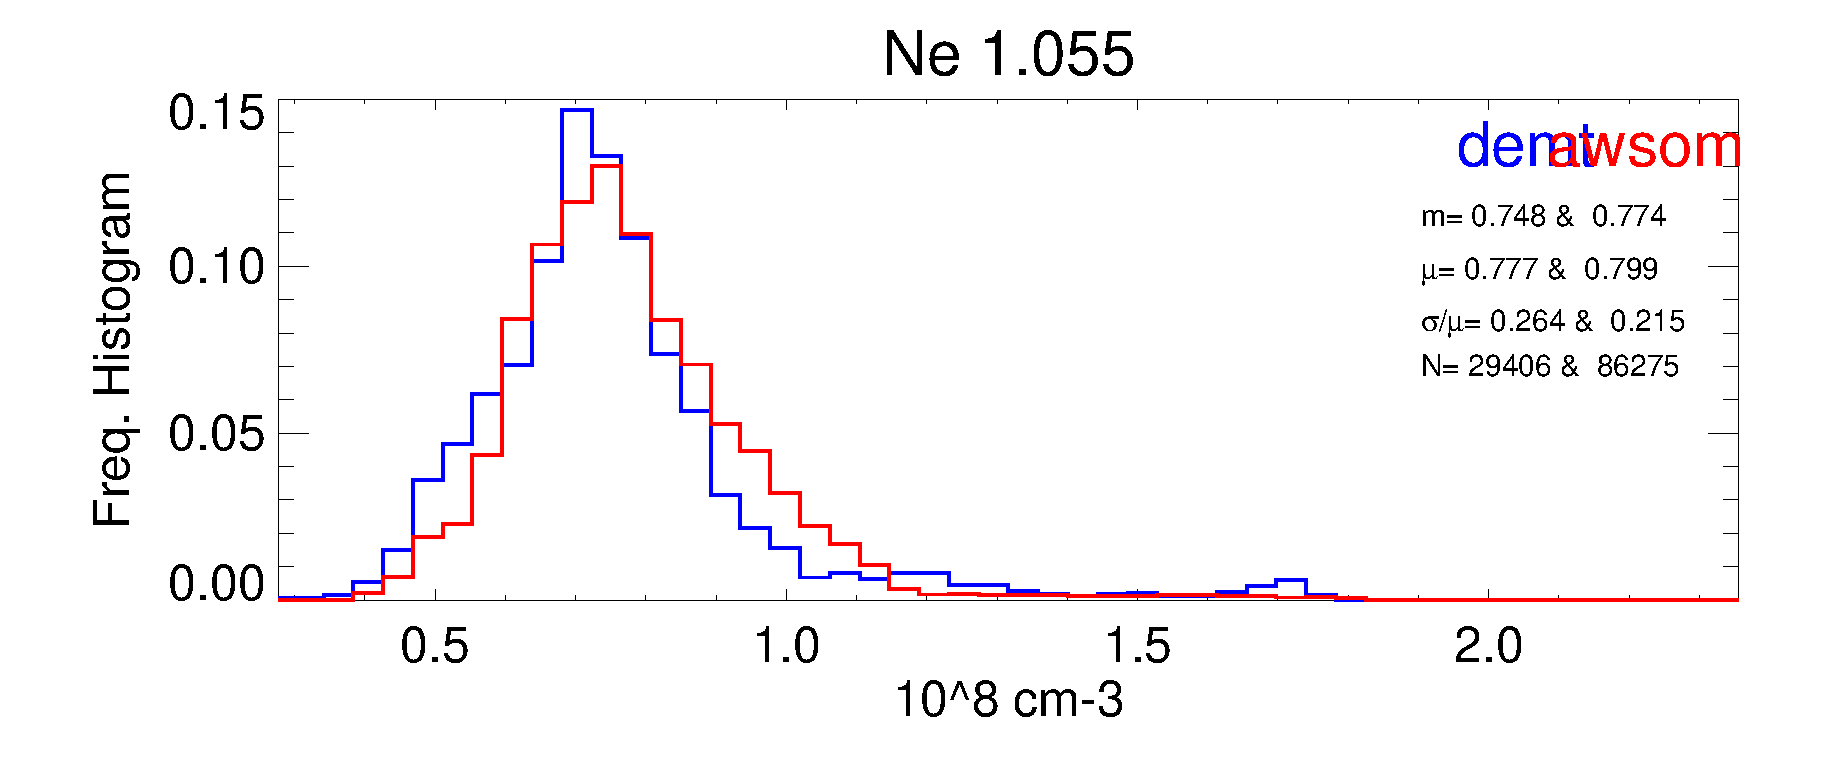
\includegraphics[width=0.32\textwidth]{figuras/proceeding_2208_demt_awsom_streamer_ne_1055.eps}
  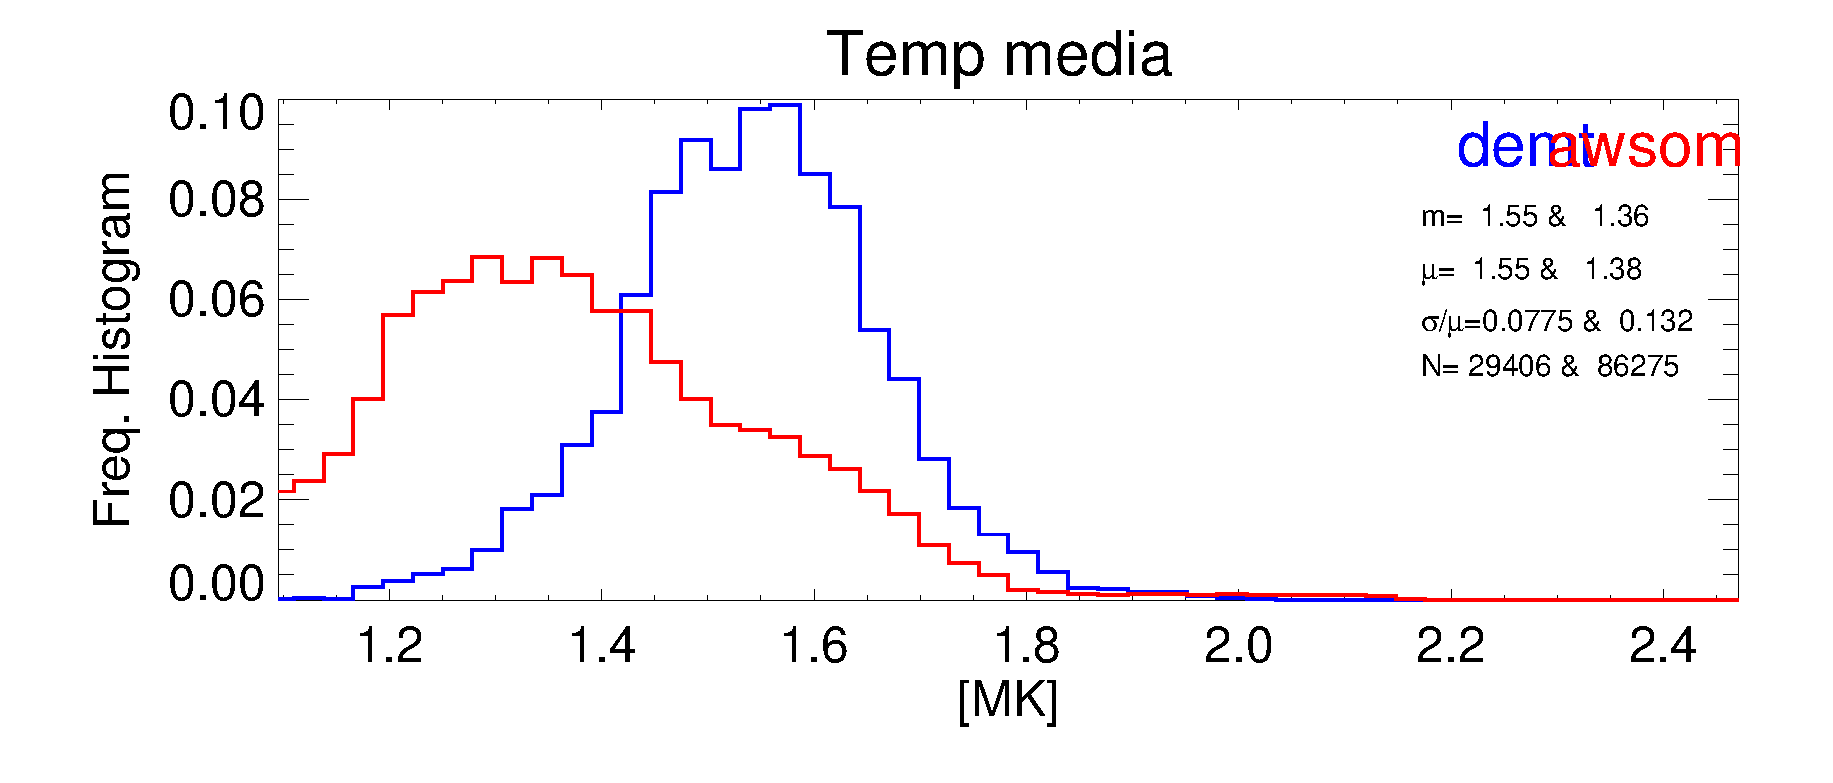
\includegraphics[width=0.32\textwidth]{figuras/proceeding_2208_demt_awsom_streamer_Tm.eps}
  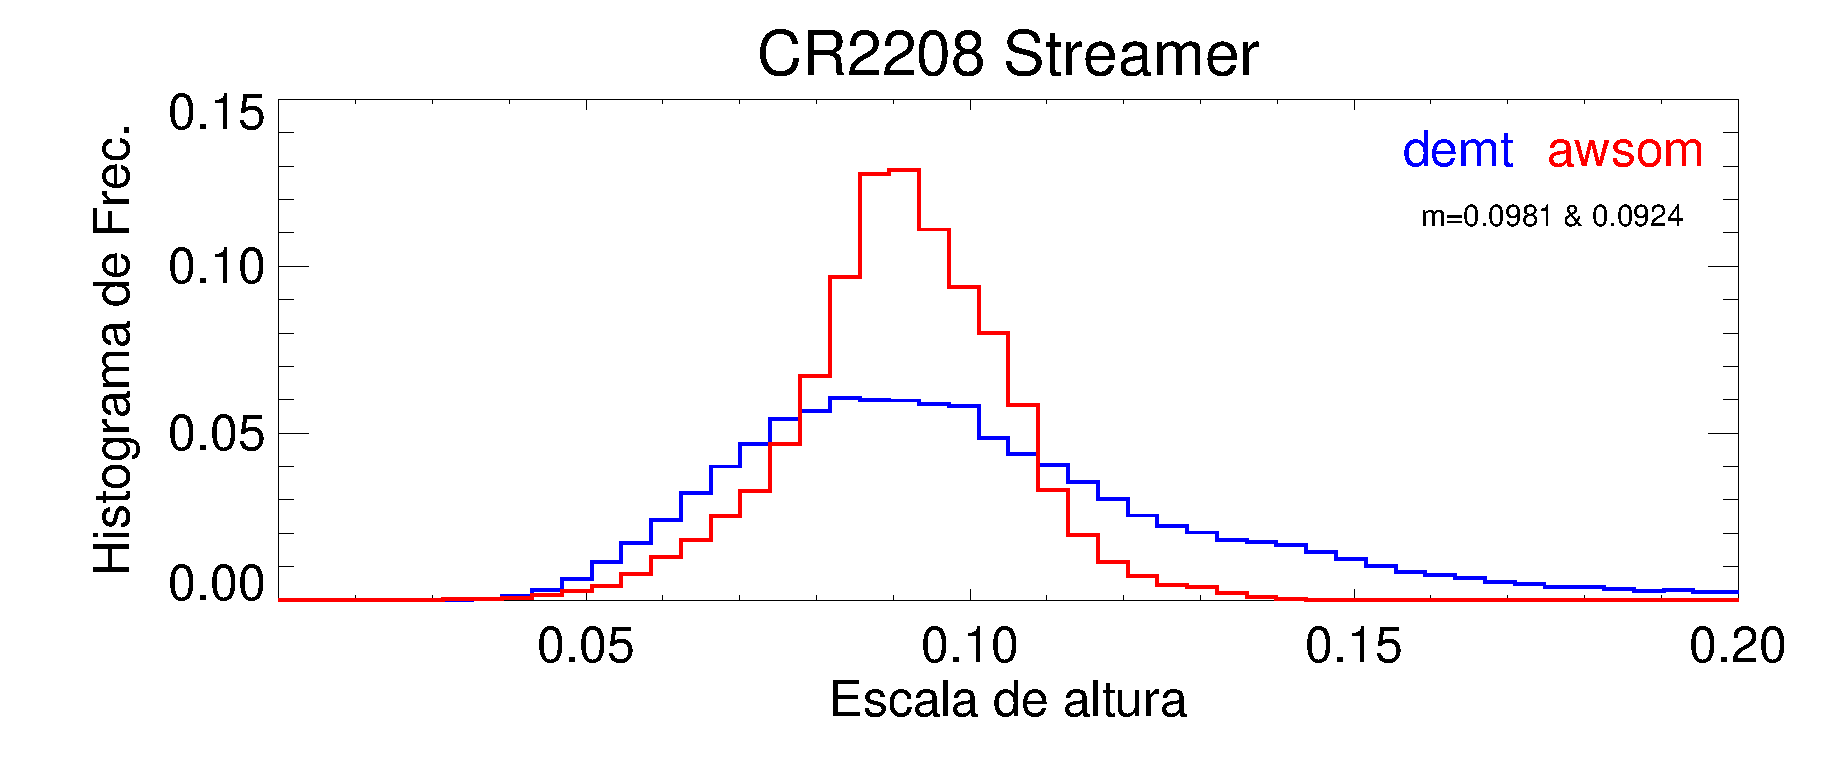
\includegraphics[width=0.32\textwidth]{figuras/proceeding_2208_demt_awsom_streamer_lambda_n.eps}
  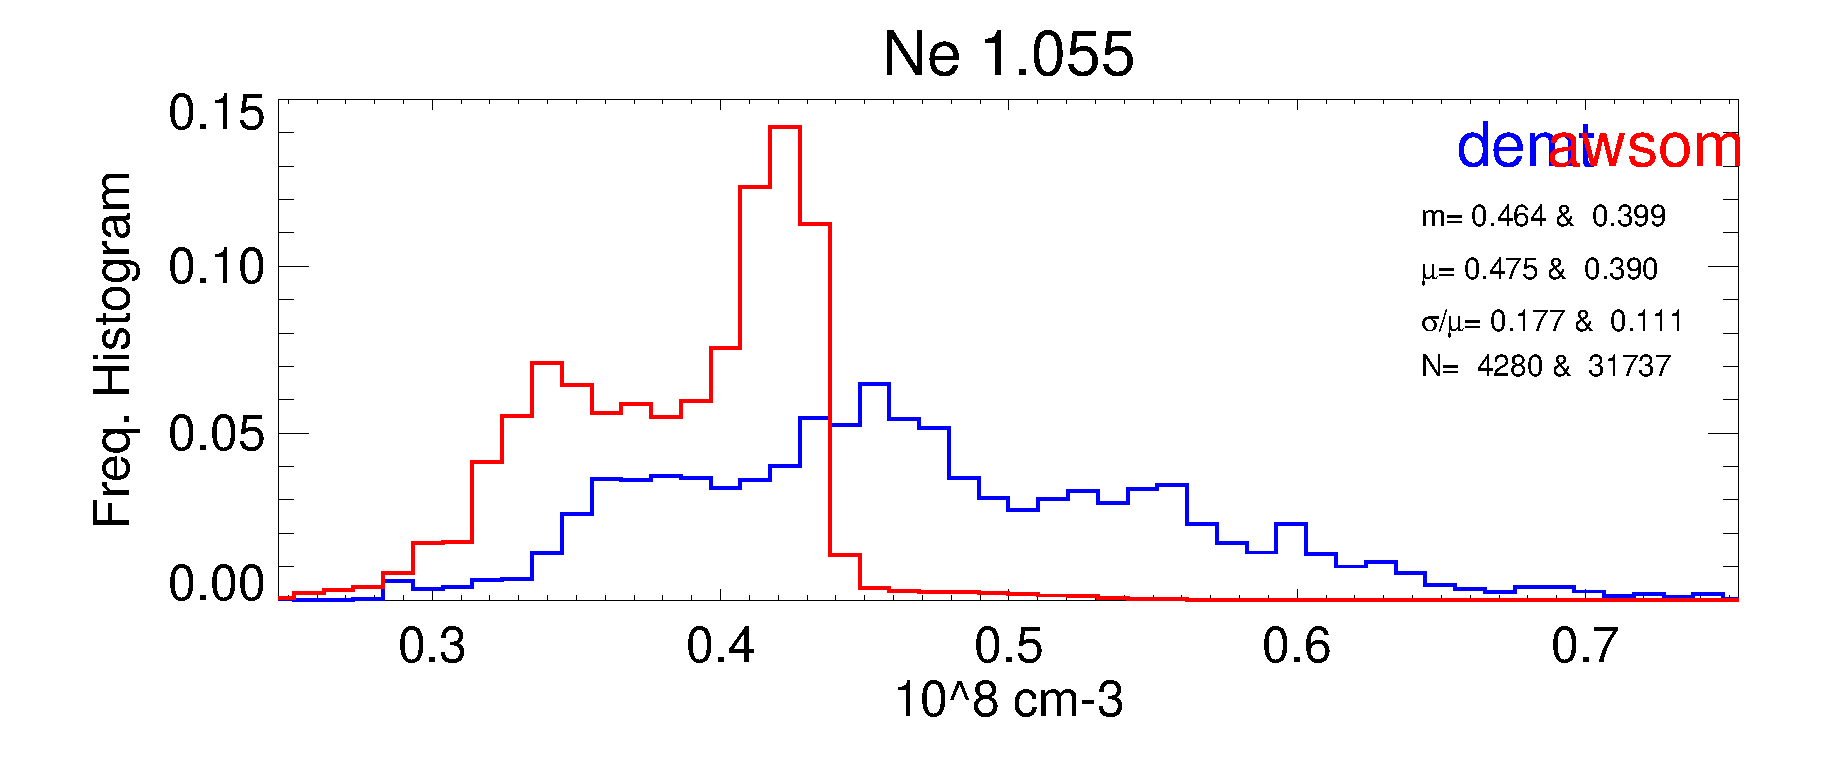
\includegraphics[width=0.32\textwidth]{figuras/proceeding_2082_demt_awsom_CH_ne_1055.eps}
  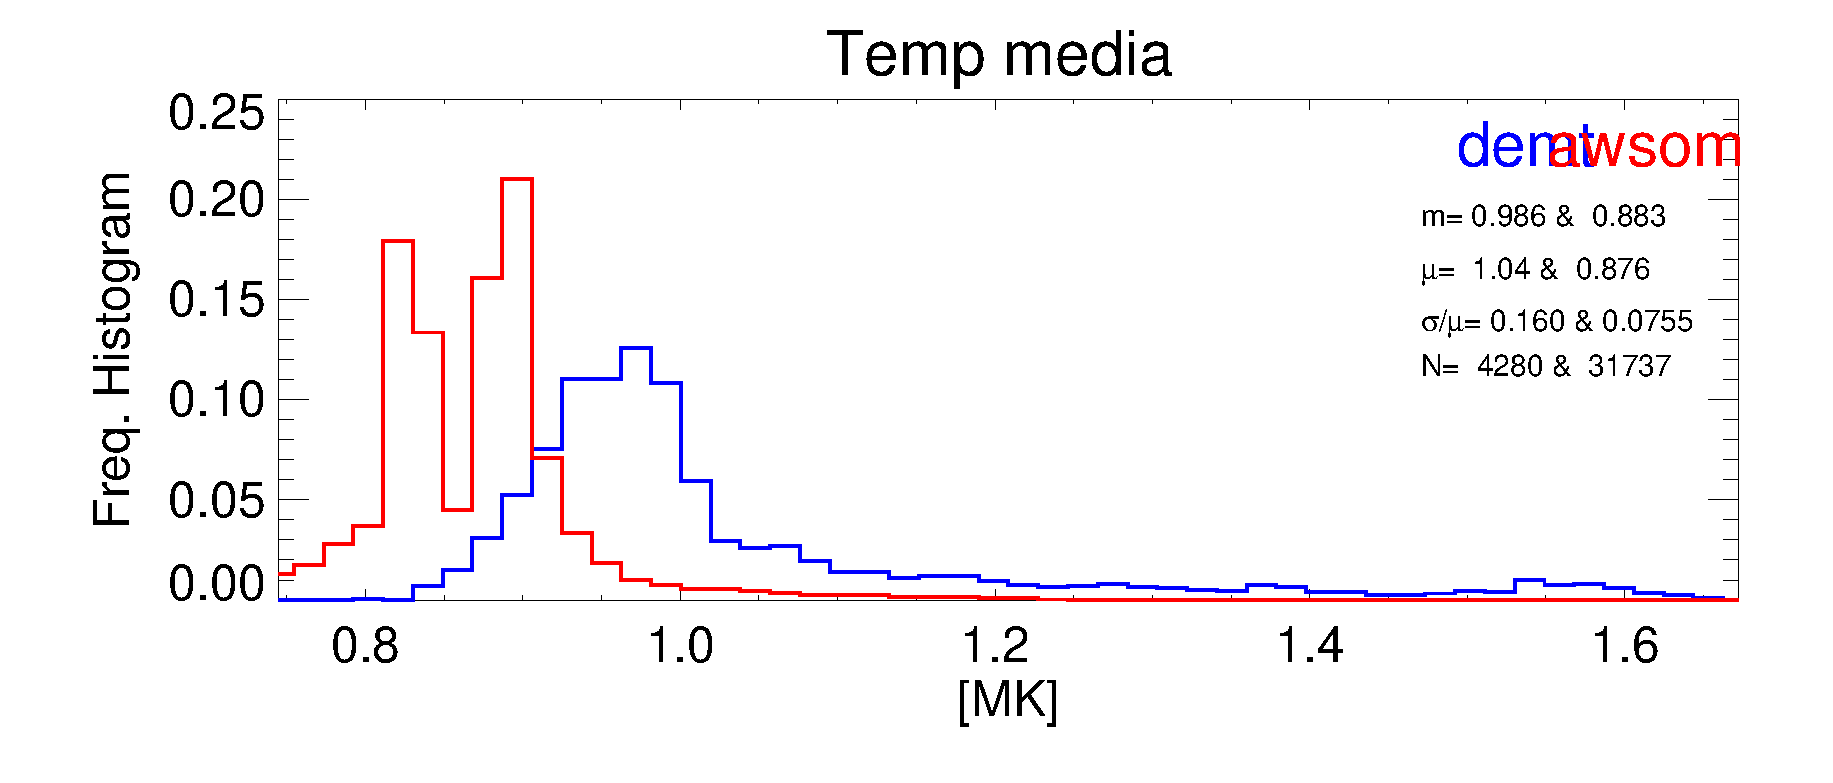
\includegraphics[width=0.32\textwidth]{figuras/proceeding_2082_demt_awsom_CH_Tm.eps}
  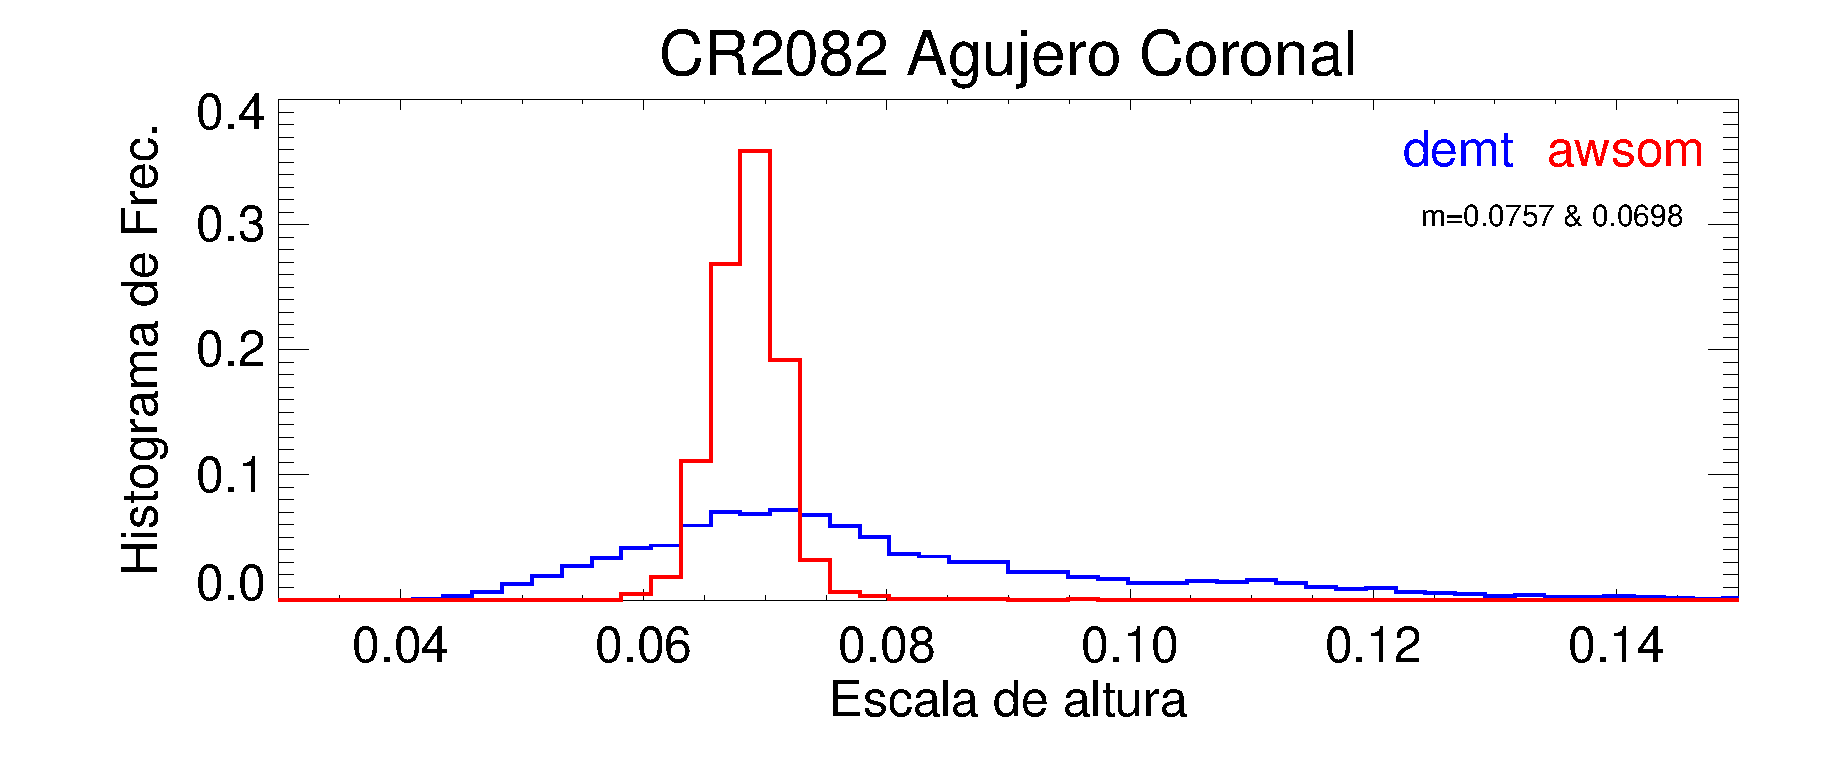
\includegraphics[width=0.32\textwidth]{figuras/proceeding_2082_demt_awsom_CH_lambda_n.eps}\\
  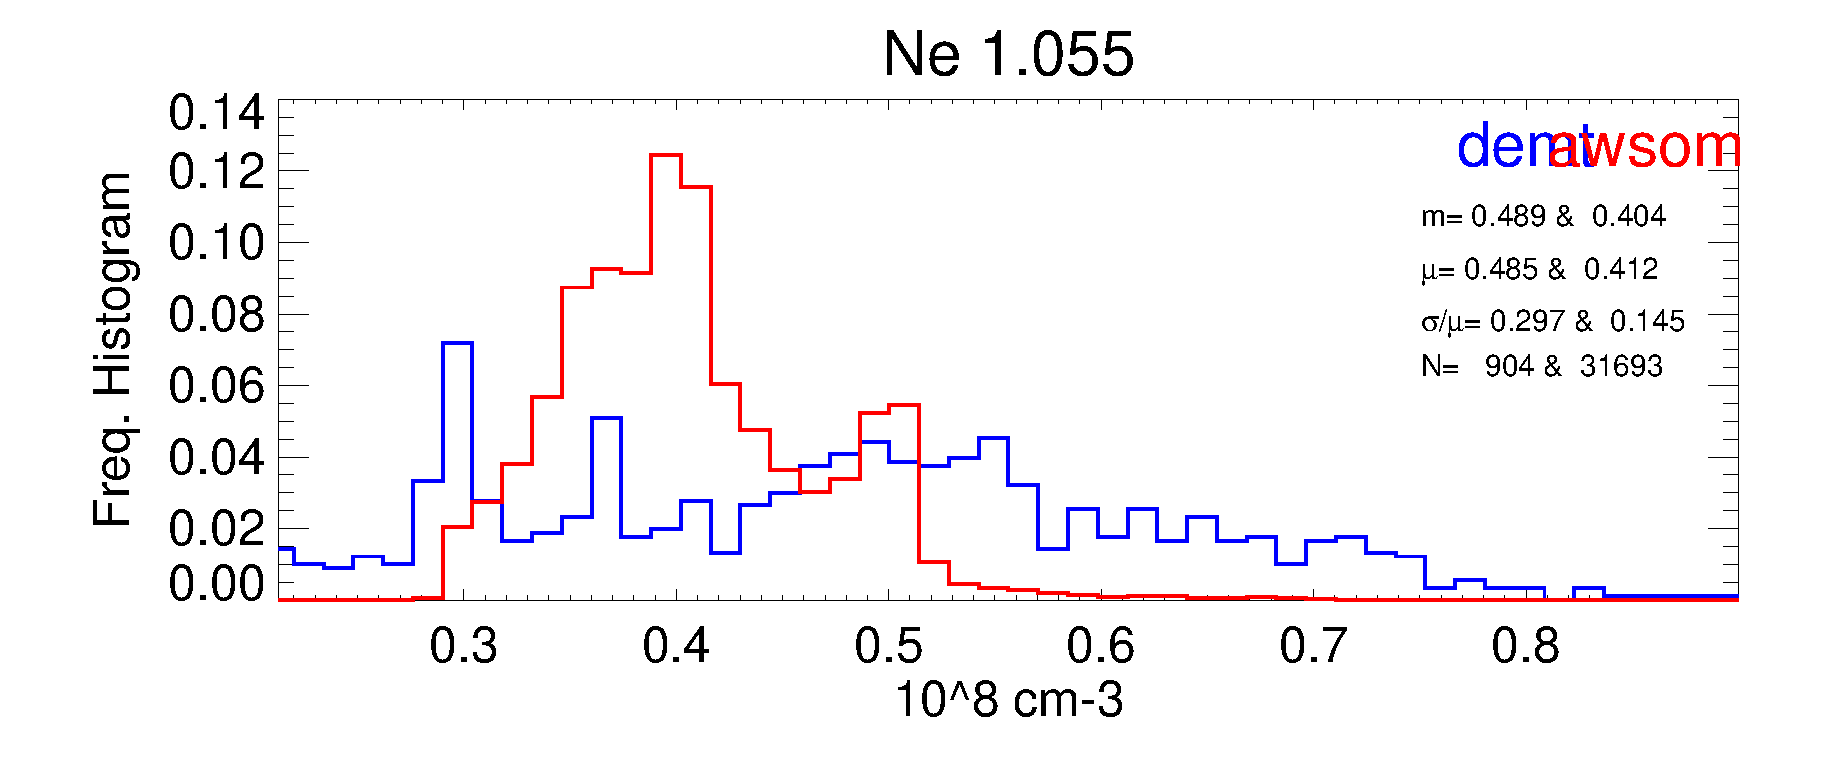
\includegraphics[width=0.32\textwidth]{figuras/proceeding_2208_demt_awsom_CH_ne_1055.eps}
  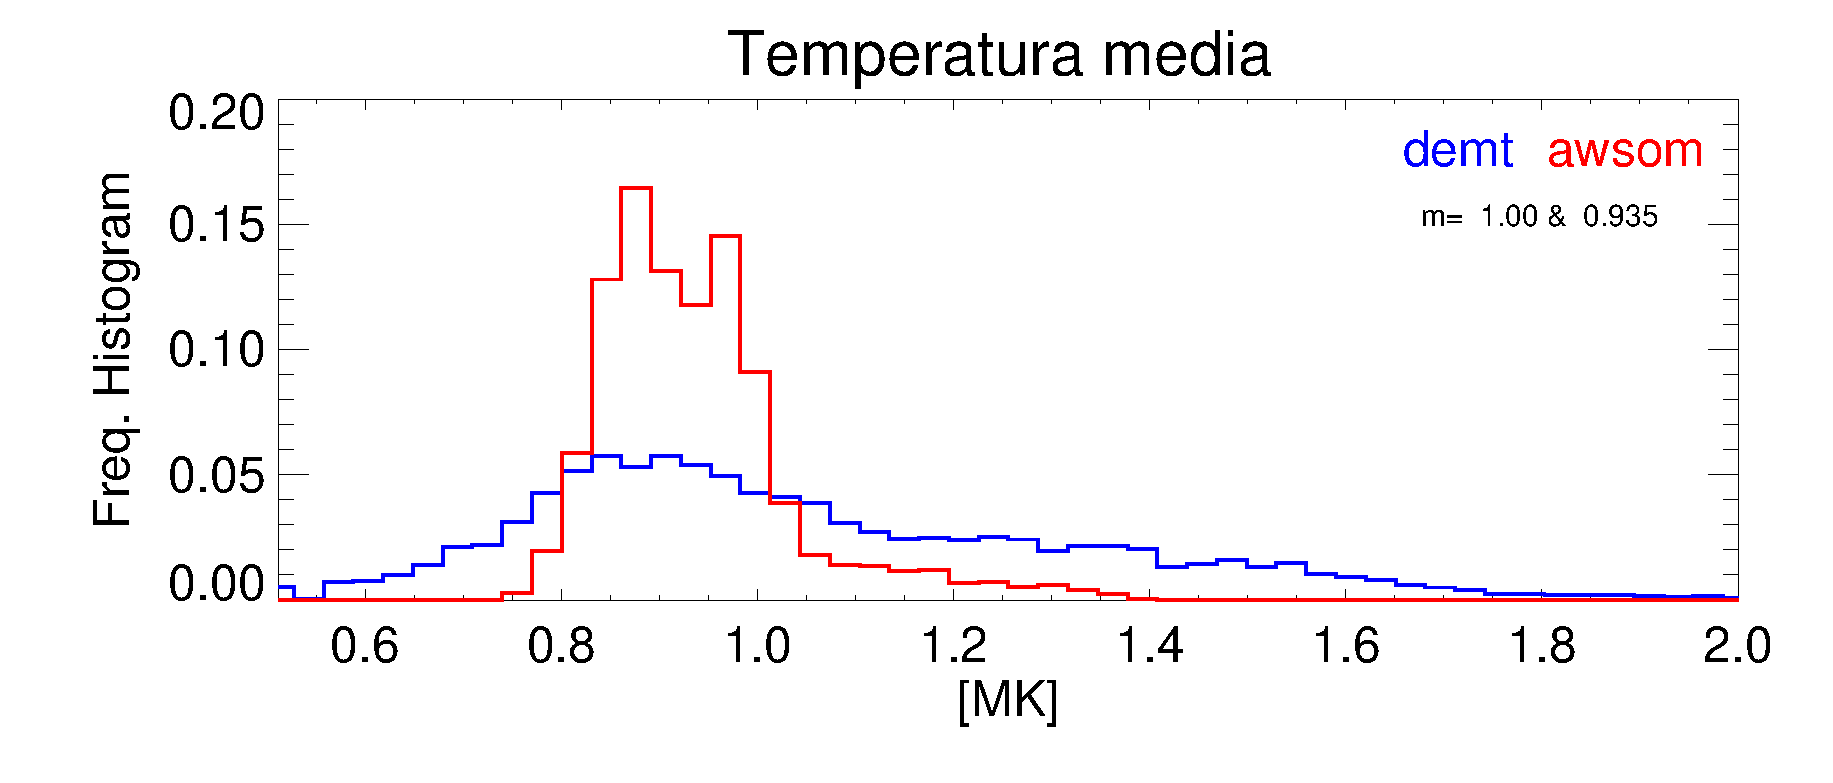
\includegraphics[width=0.32\textwidth]{figuras/proceeding_2208_demt_awsom_CH_Tm.eps}
  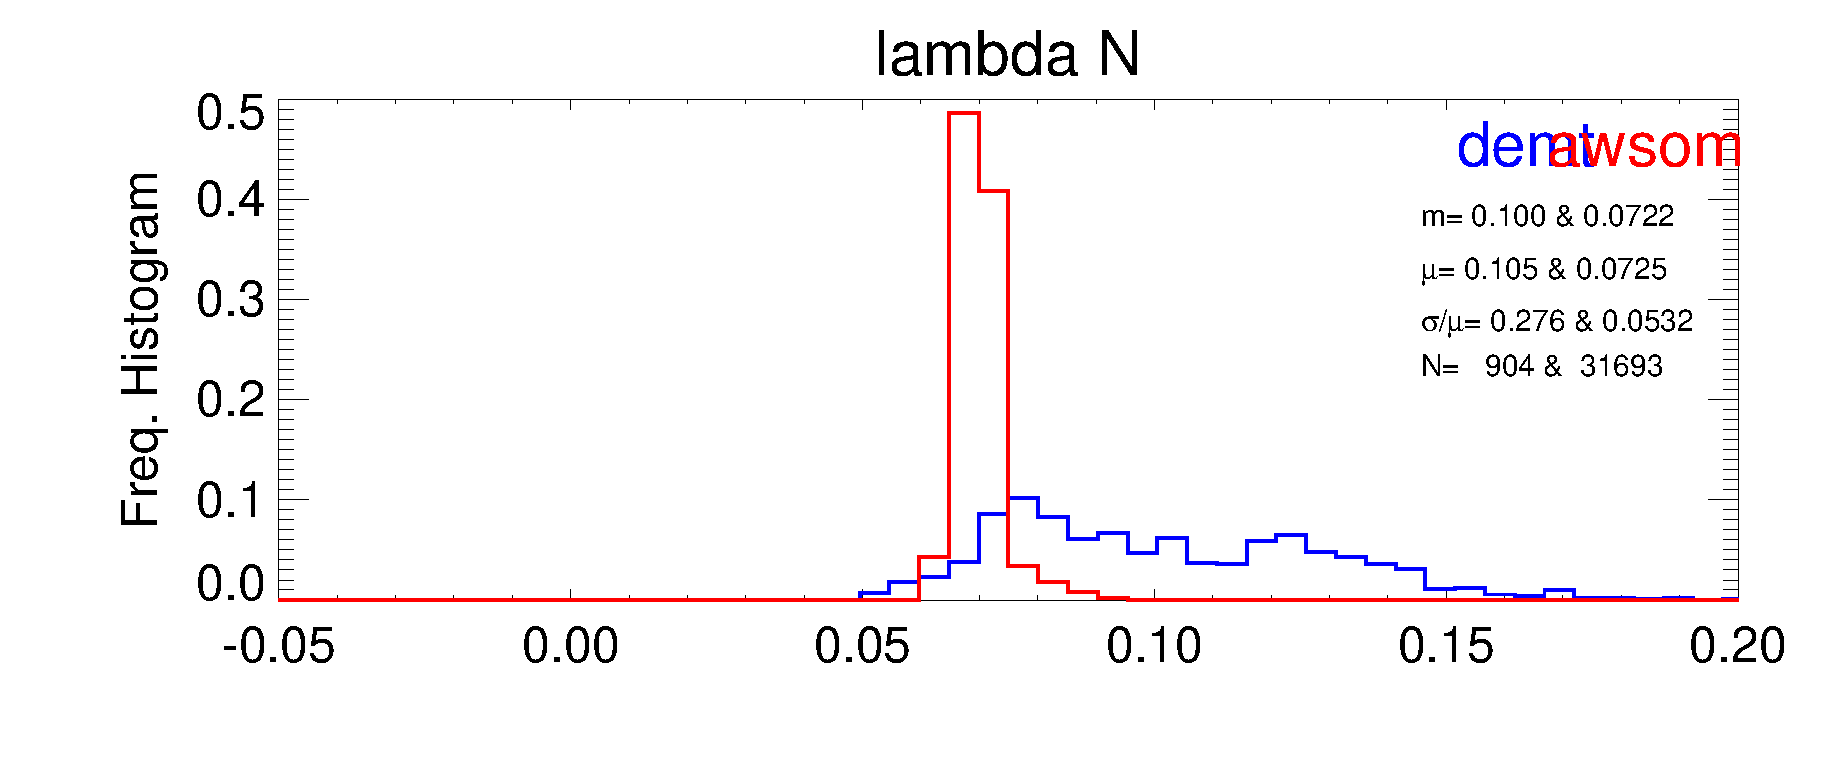
\includegraphics[width=0.32\textwidth]{figuras/proceeding_2208_demt_awsom_CH_lambda_n.eps}
  \caption{Histograma de frecuencia de CR-2082 y CR-2208 de $N_e$ a 1.055 ${\rm R_\odot}$, escala de altura de la densidad electrónica y $\left<T_m\right>$. En azul se muestran los resultados obtenidos con DEMT y en rojo con AWSoM junto con la mediana de la respectiva estadística para la region del streamer.}
  \label{fig-histos}
\end{figure*}

%\begin{figure*}
%  \centering
%  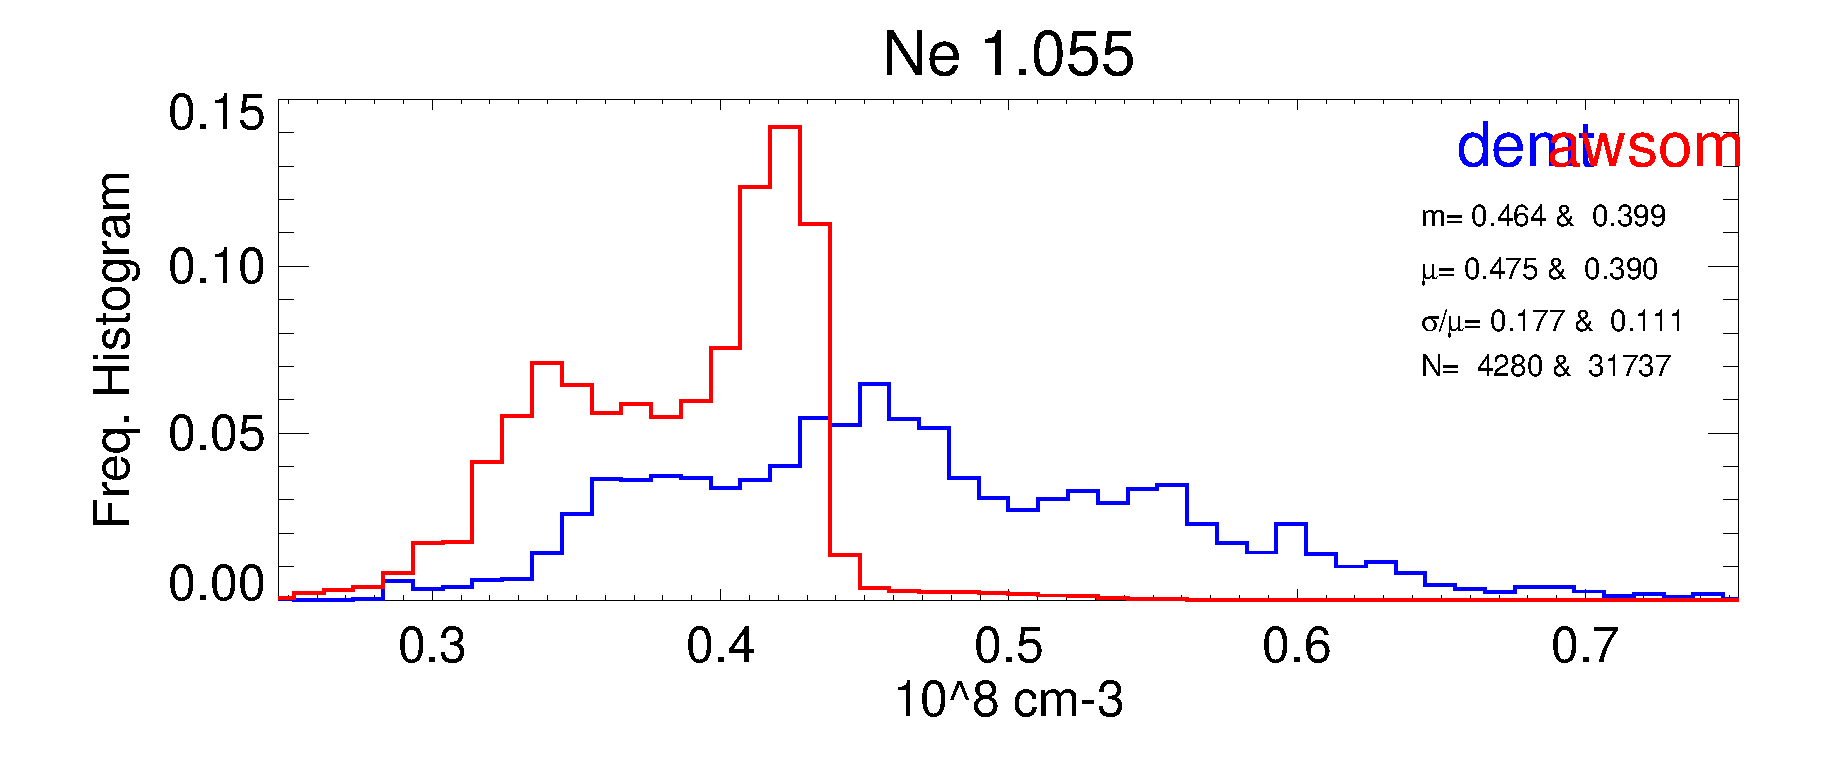
\includegraphics[width=0.32\textwidth]{figuras/proceeding_2082_demt_awsom_CH_ne_1055.eps}
%  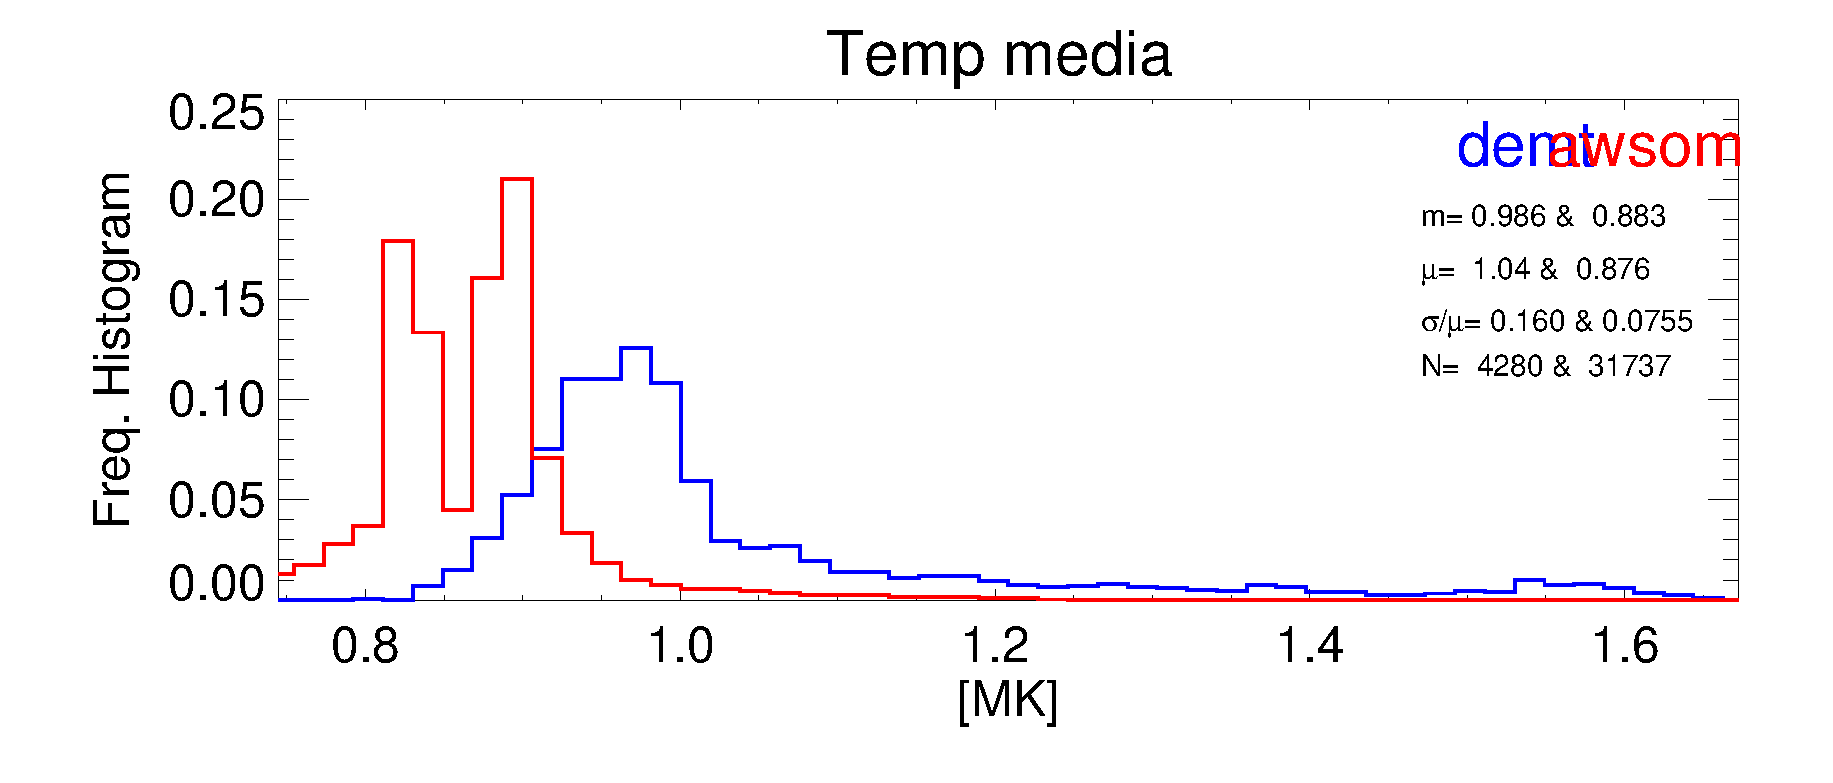
\includegraphics[width=0.32\textwidth]{figuras/proceeding_2082_demt_awsom_CH_Tm.eps}
%  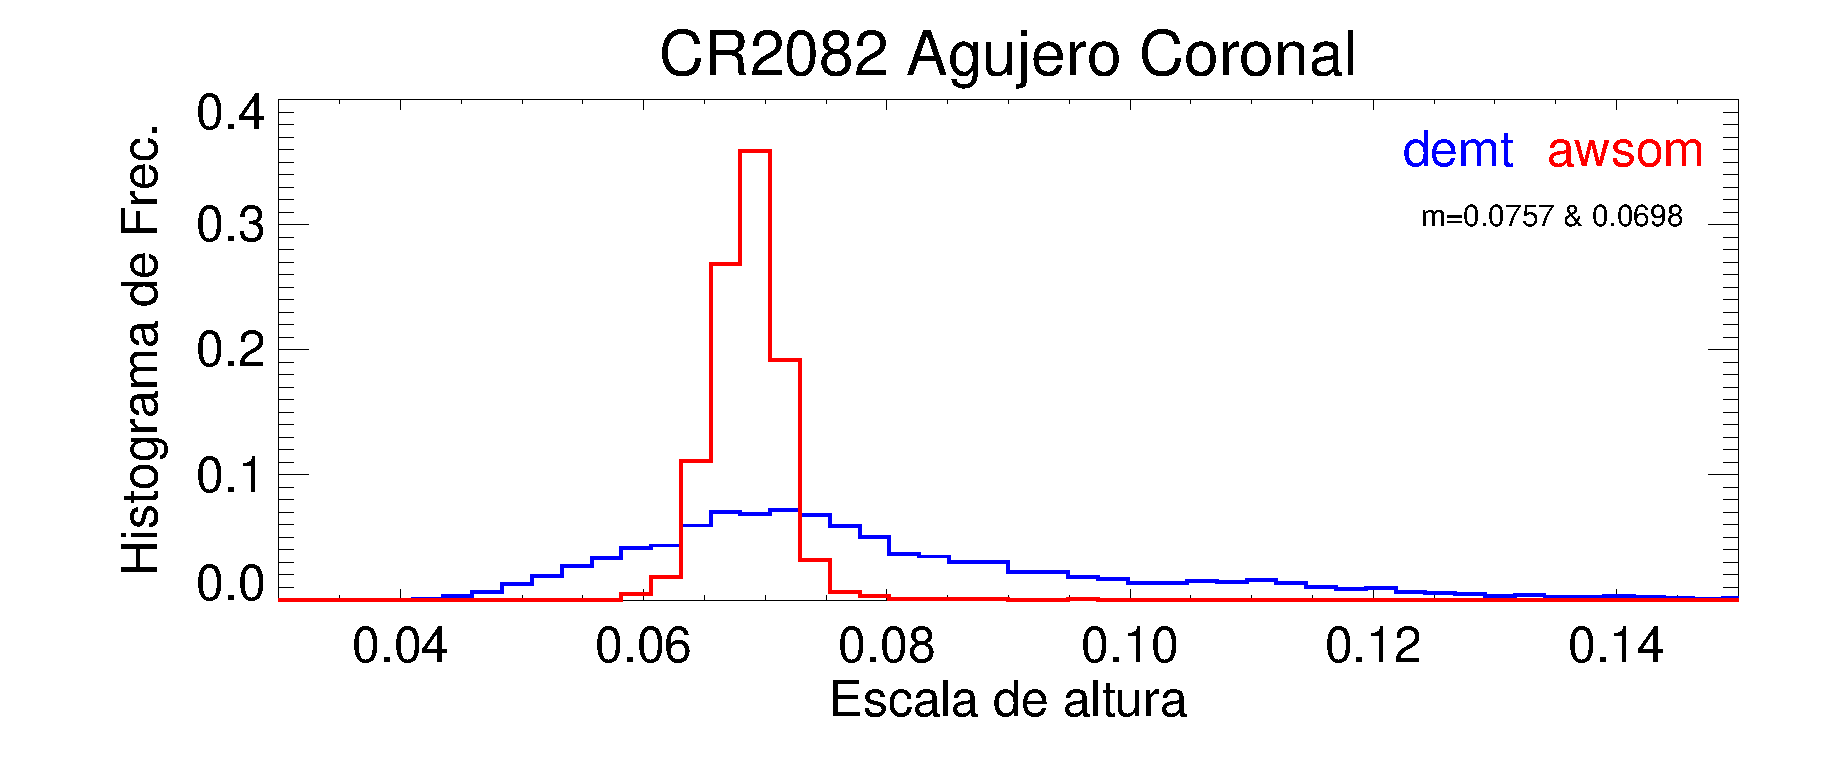
\includegraphics[width=0.32\textwidth]{figuras/proceeding_2082_demt_awsom_CH_lambda_n.eps}\\
%  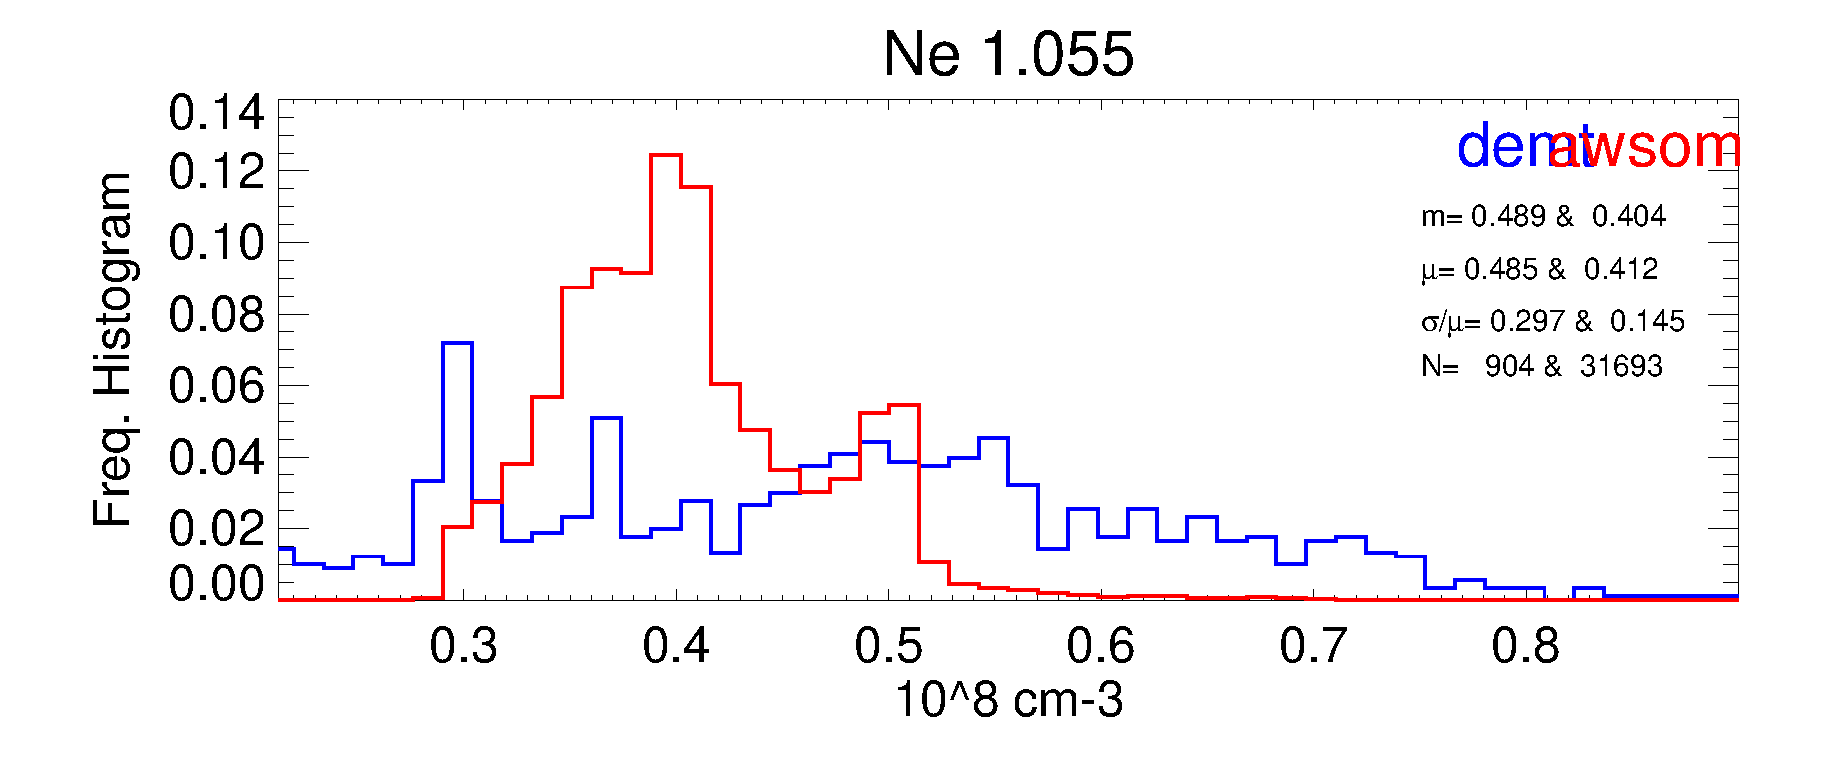
\includegraphics[width=0.32\textwidth]{figuras/proceeding_2208_demt_awsom_CH_ne_1055.eps}
%  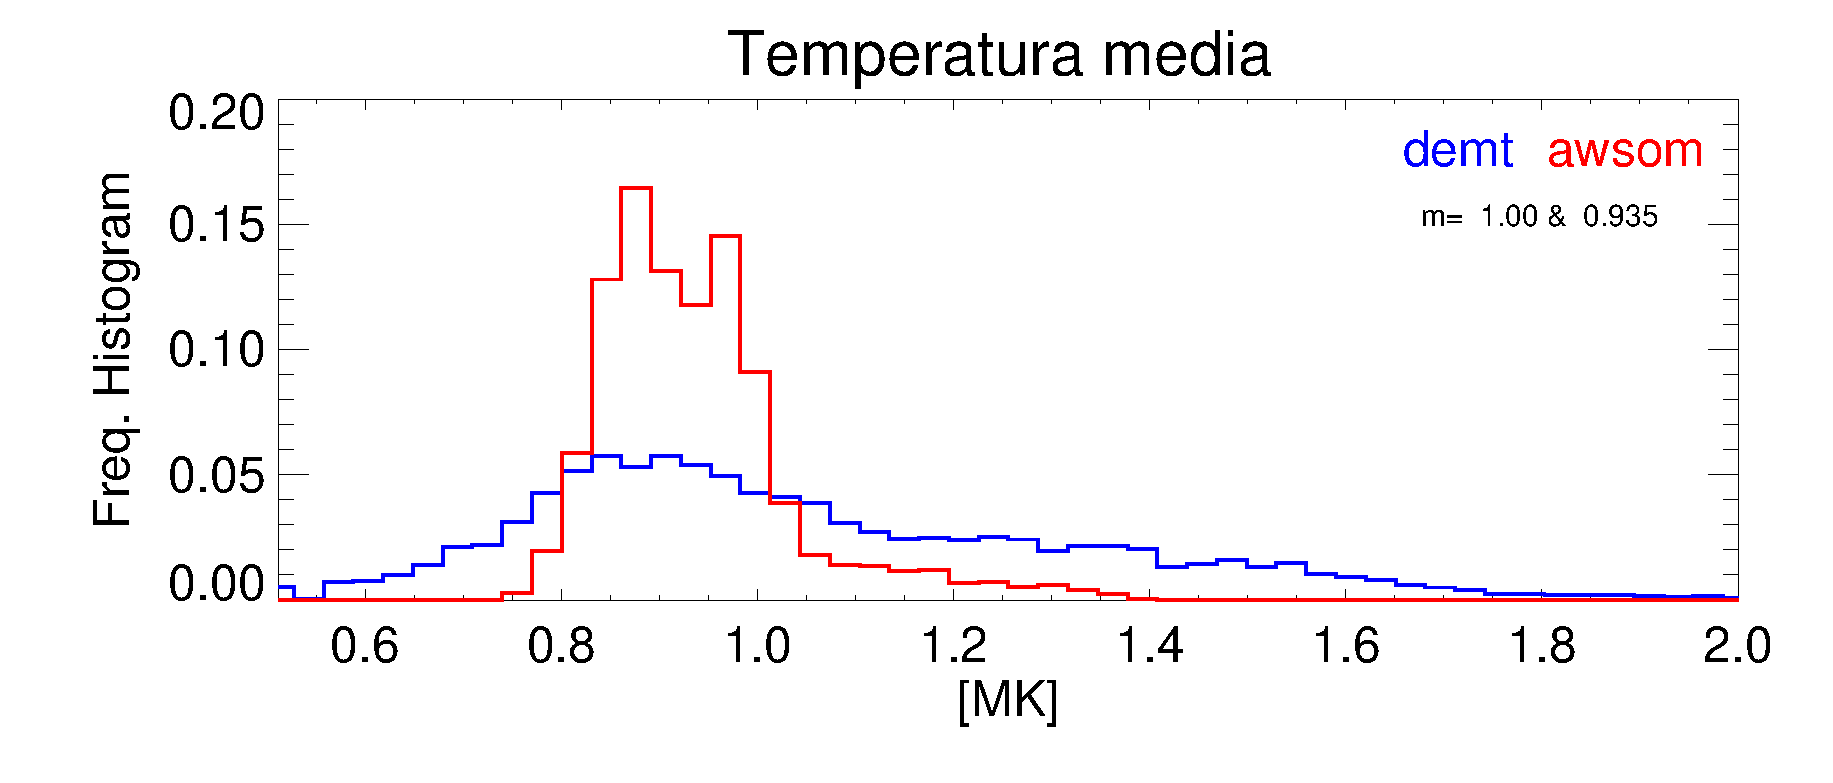
\includegraphics[width=0.32\textwidth]{figuras/proceeding_2208_demt_awsom_CH_Tm.eps}
%  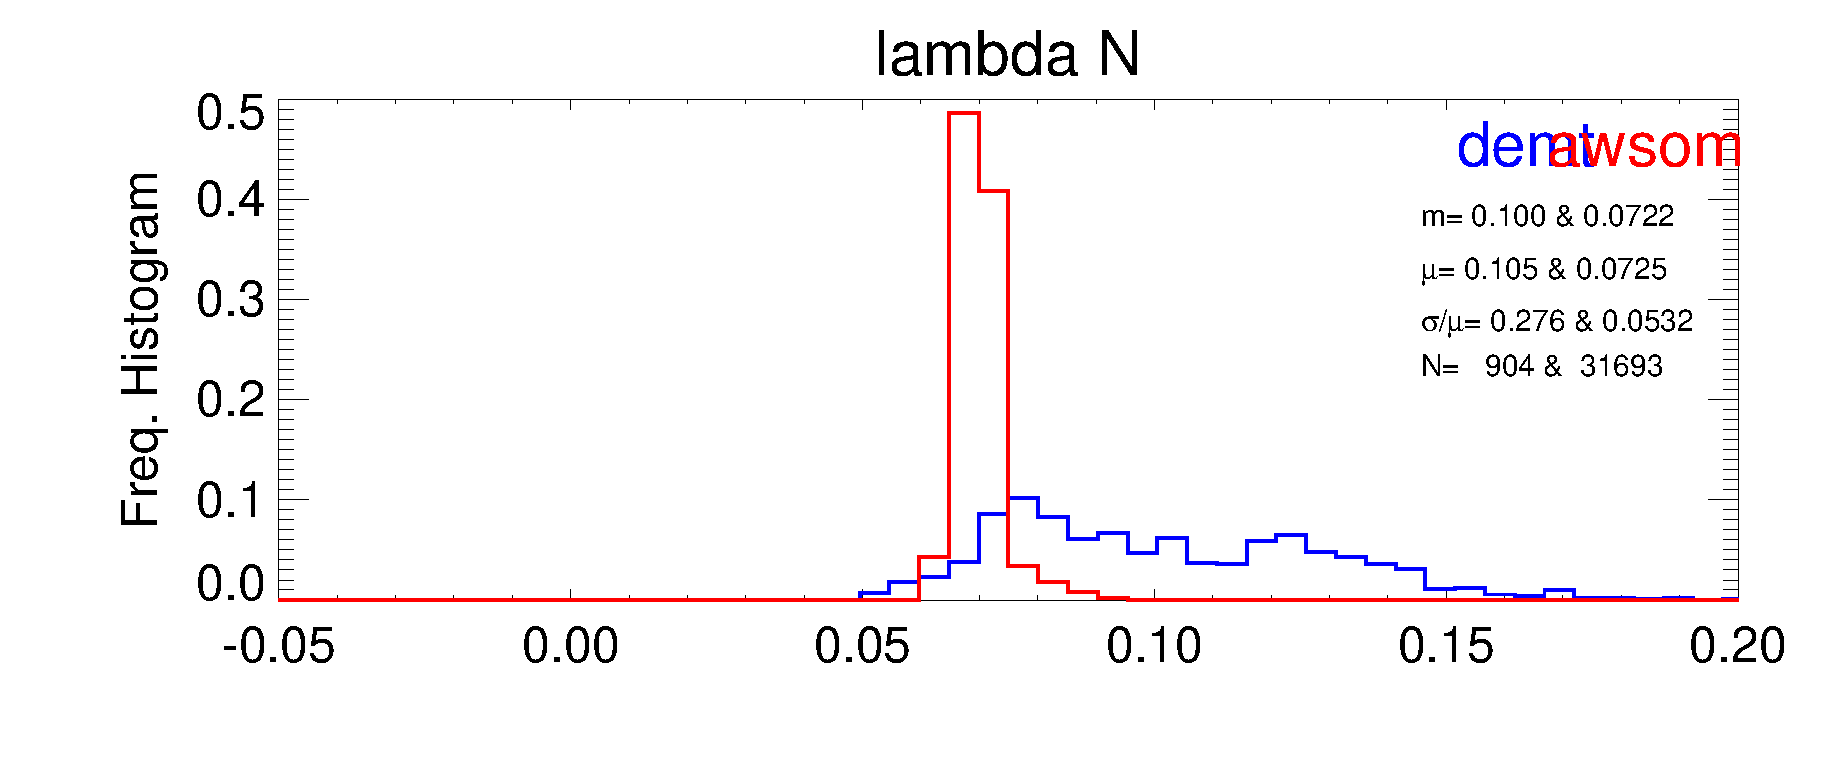
\includegraphics[width=0.32\textwidth]{figuras/proceeding_2208_demt_awsom_CH_lambda_n.eps}
%  \caption{Histogramas}
%  \label{fig-histos2}
%\end{figure*}

\section{Discusión y trabajo futuro}
*QI no estan
*down loops no estan
*modela bien dentro del 30%
*Se va a hacer una anlisis mas refinado, que involucra energia y comparaciones mas refinadas.

\begin{acknowledgement}
\texttt{A Juan roberto Macri}
\end{acknowledgement}

%%%%%%%%%%%%%%%%%%%%%%%%%%%%%%%%%%%%%%%%%%%%%%%%%%%%%%%%%%%%%%%%%%%%%%%%%%%%%%
%                                                                            %
%  Por favor no modifique las líneas de la bibliografía, salvo el nombre     %
%  el archivo de Bibtex con la lista de citas (sin la extensión .BIB)        %
%                                                                            %
%  Please do not modify the following lines, except the name of the Bibtex   %
%  file (whithout the .BIB extension)                                        %
%                                                                            %
%%%%%%%%%%%%%%%%%%%%%%%%%%%%%%%%%%%%%%%%%%%%%%%%%%%%%%%%%%%%%%%%%%%%%%%%%%%%%% 

\bibliographystyle{baaa}
\small
\bibliography{baaa61b_2020_dglloveras}
 
\end{document}
